%\pagestyle{article}
\documentclass[a4paper]{article}
\usepackage[english]{babel}
\usepackage[utf8]{inputenc}
\usepackage{graphicx} % for figures
\usepackage[section]{placeins} %This prevents placing floats before a section.
\usepackage{csquotes}

\usepackage{natbib}% better citation
%\usepackage{hyperref} %autoref
\usepackage[hidelinks]{hyperref} %hidelinks to remove ugly blue format
\usepackage{amsmath} % for \tag and \eqref macros in mathematical eq.


%% Sets linestretch, paragraphstrech, indentation and footnote stuff 
\usepackage{parskip} %space between paragraphs
\parskip=12pt %set space between paragraphs
\setlength\parindent{12pt} %paragraf indentation
\usepackage[onehalfspacing]{setspace} %linespacing; does not affect footnotes
\setlength{\footnotesep}{0.7\baselineskip}% space between footnotes
\usepackage[hang,flushmargin]{footmisc} %% removes identation in footnoteshttps://www.overleaf.com/project/5b98e00a21d3bd15ac5a2e86

\usepackage{makecell} % make cells in tabels for longer text

\usepackage[colorinlistoftodos]{todonotes}

%% For header and footer (1)
% Marco
\usepackage{fancyhdr}
\pagestyle{fancy}
\textwidth = 424pt % test width ish
\oddsidemargin = 18pt % margin width ish

\fancyheadoffset{0 in} % Shifty solutions..

\fancyhf{} %% clear defuelt header and footer

%% For header and footer (2)
%Specifics
\lhead{Simon P. von der Maase}
\rhead{\today}

\lfoot{University of Copenhagen}
\rfoot{\thepage}
\renewcommand{\footrulewidth}{0.8pt}

\title{Where Men Rebel\\A Modern Approach to Conflict Forecasting}

\author{Simon Polichinel von der Maase}
\date{January 2019}

\begin{document}

	\begin{titlepage}
		\maketitle
		%Character count: 43.950/44.000\\
		\noindent\rule{\linewidth}{0.4pt}
		\begin{figure}[h]
			\centering
			
\includegraphics[scale=0.32]{KU_logo.png}
		\end{figure}
		\thispagestyle{empty} % removes page number on front page
	\end{titlepage}
    \tableofcontents
\pagebreak

\begin{abstract}
\todo[inline]{to come}
\textbf{Reading Companion}: Til Frederik, og hvem der ellers måtte være interesseret. Jeg har mest fået arbejdet på de ting vi snakkede om sidst, så det er også det jeg gerne vil havde feedback på. Mere specifikt vil jeg gerne vide: Er opbygningen mere tydelig nu? Er målet mere klart (bla. med nyt research question)? Vil du/I stadigt gerne have afsnit 3 "The Present Challange" længere frem? Synes du/I jeg kan undvære hele afsnit 2 hvis jeg skriver lidt mere om de to udviklinger (developments) i introen (hvor jeg nævner dem alligevel)? I afsnit 3 synes du/I nu giver en bedre priming til afsnit 4.2 om Gaussian Processes?\par\par

Kort sagt: Giver det mere mening nu? Føler I jer mere taget i hånden?\par

\end{abstract}
\pagebreak

\section{Introduction}
\todo[inline]{The World}

\begin{displayquote}
\emph{[...] the estate of Man can never be without some incommodity or other; and [...] the greatest, that in any form of Government can possibly happen to the people in generall, is scarce sensible, in respect of the miseries, and horrible calamities, that accompany a Civill Warre;} \cite[128]{Hobbes_1991}\par
\end{displayquote}

Civil wars, and internal conflicts in general, have plagued mankind throughout the ages. And still, this affliction has not yet been throttled. Since 1960, over half of all nations have experienced some manner of internal conflict leading to fatalities \citep[3-4]{Blattman_Miguel_2010}. Indeed, since the end of the Second World War intra-state conflicts have been far more common than inter-state wars and over five times as many people have died in intra-state conflicts compared to inter-state wars \citep[563]{Collier_Hoeffler_2004}. Thus the 367 years old quote above is today as relevant as ever.\par

\textbf{This thesis represent a substantial step towards the construction of a reliable computational framework for predicting future conflicts at a sub-national level. A so called \emph{early-warning system}.} In the short run such system will provide international actors valuable information and time to act; mitigating the fallout of conflicts \citep{Ward_Greenhill_Bakke_2010, perry_2013}. In the long run such system will generate theoretical insights into the mechanics of conflicts potentially enabling actors to addresses the underlying courses \citep{Schrodt_2014, chadefaux2017conflict}. Given these huge potentials, efforts to create an early-warning system have been called the "conflict researchers’ ultimate frontier" \citep[474]{cederman2017predicting}. As such the contribution of this thesis is highly topical and can provide practical and ongoing guidance in future conflict prevention, intervention and peace keeping efforts.\par

A complete early-warning-system would be constituted by a legion of sophisticated components. In this thesis I will focus on one of these components: A component capable of using past patterns of conflict to predict future patterns of conflicts. The reason I choose this focus is, as I will demonstrate throughout this thesis, that this approach has a number of vary appealing properties such as a clear theoretical foundation, high prediction power and takes advantage of very current data. As such, using past patterns for future prediction has the potential of being on of the most important and central components of any complete early-warning-system. This makes this approach an relevant and worthwhile subject for the thesis at hand.\par

%Specifically [...]
%\todo[inline]{The specific steps, and prime conclusions of this thesis will be briefly outlined here.}

The proceeding subsections outlines some prime insights, conclusion and challenges regarding conflict forecasting in general. This concurrently qualifies and explains why I focus on the paste patterns as oppose the e.g. structural prerequisites. The purpose is to prime the way for a more in-depth presentation of the project at hand.\par

\subsection{Conflict prediction so far}
% condensat af lit review
%\todo[inline]{The science}
%\todo[inline]{Skal omskrives så det passer til ny struktur.}

% what
The study of internal conflicts has a long and rich history. The sub-field of computational conflict prediction\footnote{from here just denoted conflict prediction} is a rather novel offspring. Researches of conflict prediction uses modern computational tools in effort to predict the time and place of future conflicts \citep{cederman2017predicting, chadefaux2017conflict}. Some of the earliest examples in academia of such focus being \cite{Goldstone_2010}, \cite{Hegre2013} and \cite{perry_2013}.\par

% why not before
There are two main reason why the field of conflict prediction - despite its obvious usefulness - has not flourished before. First of all; the required technology is rather new. Indeed, some of the more impressive recent results is due to novel developments in quantitative methods, computation power and data availability \citep{ol2010afghanistan, perry_2013}. Secondly, traditional conflict research has focused on causes, correlates and prerequisites of conflict rather than generating actual predictions \citep[8]{chadefaux2017conflict}. As such, modern predictive efforts are still regarded with high skepticism and papers devoted to prediction have been accused of lacking strong theoretical grounding \citep[8-9]{chadefaux2017conflict}. 

% why it should be now - det her gentager du længere ned... kort det her.
In reality, however, both prediction and explanation are important components of scientific inquiry, and both are needed to generate and test theories \citep{Schrodt_2014, chadefaux2017conflict}. Indeed, in the natural sciences, accurate predictions is central for the validation of theory \citep[289]{Schrodt_2014}. As such, the restraint against predictions in the field of conflict research have been increasingly criticized \citep{King_Zeng_2001, Ward_Greenhill_Bakke_2010, Goldstone_2010, Schrodt_2014, chadefaux2017conflict}. What more is; creating models with actual prediction-power will also provide heuristic tools and powerful policy-guides for real world application \citep[372]{Ward_Greenhill_Bakke_2010}.

% another recent development: disaggregation.
Another recent development in the field of conflict studies and conflict predictions alike is the shift from countries to more disaggregated geographical units of analysis. Countries have traditionally been the main focus, but since the phenomena we are investigating is a sub-country phenomena, the unit of analysis should also be disaggregated at sub-national level \citep[490]{Cederman_Gleditsch_2009}. Employing a disaggregated unit of analysis allows me to create a more detailed analysis of conflict patterns. It also allows my to better analyses incidents where administrative boarders provide little to no ward against conflict diffusion \citep[445-446]{ol2010afghanistan}. In turn, the derived insights allows me to generate forecastings pertaining to specific sub-national regions rather then entire countries.\par

% the last recent development: Structures to patterns.
The last development I shall tuch upon here constitutes more directly the starting point of this thesis. This development concerns the turn from structural data to event data. Structural data being data pertaining to poverty, deprivation, resources, political regimes ect. And event data being data pertaining to the patterns of past conflicts.\par 

Traditional efforts have tended to use structural features as foundation. This has been true for estimations and predictions alike \cite[10]{chadefaux2017conflict}. However, in a recent contribution of my own I have shown that patterns of conflict events in themselves appears to hold much more prediction power than the traditional structural variables \citep{Maase}. These findings aligns perfectly well with a growing strain of the literature concerning conflict diffusion and cognition. Little doubts remain that conflicts cluster in time and space \citep[15]{crost2015conflict}. Furthermore, recent efforts have shown that the clustering and diffusion of conflict is often a direct product of contagion \citep{buhaug2008contagion,schutte2011diffusion,crost2015conflict,bara_2017}. As such, when it comes to sheer prediction power event data appears to have the advantage over structural data. 

Importantly, event data is also, at present, much more current and more often maintained than the data pertaining to the structural features. In practise this means that the data I use for actual forecasting is much closer in time to the forecastings I wish to generate, thus creating more reliable predictions and mitigating uncertainty. A further substantial advantage of event data over structural data.\par

Given these insights and conditions - and the scope of the thesis at hand - I will only utilize data relating directly to conflict events in this prediction effort. That is; estimating the probability of future conflicts given past patterns of conflict.\par

The next section will introduce the concrete contribution of thesis in broad terms. That is; a framework for constructing reliable conflict forecastings using the temporal and spatial pattern of past conflicts.\par

\subsection{This framework}
\todo[inline]{this paper}

% what you gonna do there champ?
The prerequisite for using past patterns of conflicts to predict future patterns of conflict is the ability to identify and extract salient patterns and further extrapolate said patterns into future years. In this thesis I will show how this can be done using the machine learning technique of \emph{Gaussian processes}. Furthermore, I will demonstrate how the technical properties of Gaussian processes aligns remarkable well with the theory foundation of conflict diffusion in general. The presentation, qualification and exemplification of how Gaussian processes can turn past conflict patterns into future conflict predictions is the prime objective of this thesis.\par

% RQ
The research question motivation this thesis can be summed up accordingly:\par

\begin{displayquote}

\emph{\textbf{Research Question:} How can we use the temporal and geo-spatial patterns of past conflicts to forecast and predict the time and place of future conflicts?}\par

\end{displayquote}

% Data and unit of analysis
To convey how I will answer this question, I will start by introducong the data used. To identify the patterns of conflict I need data pertaining the time and place of past conflicts. For this i use data from the Uppsala Conflict Data Program \citep{UCDP_2017}. This data denotes, among other things, conflict fatalities at specific coordinates and dates \citep{UCDP_2017}. I take the logarithm of this measure to create a measure of \emph{conflict magnitude} (cm). The temporal dimension spans from 1989 to 2017 and I aggregated it at a yearly level. The spatial dimension I aggregate using a global grid constituted by $0.5 \times 0.5$ decimal degree cells; that is squares roughly measuring $50km\times50km$ at the equator \citep[367]{Tollefsen_2012}. Thus, the unit of analysis is one specific grid cell, pertaining to one specific year.\par

% Time lines as functions
I will refer to the combined observed years of a given cell as the \emph{time-line} of that cell. Each time-line tells the story of conflict in the corresponding cell through the years. Each time-line can also been seen as a continuous function $y = f(x) + \epsilon$ where $\epsilon$ is a noise term, $y$ is conflict magnitude and $x$ is years. If we could estimate this function we could also extrapolate it into future by introducing new years; $x_{new}$. This is exactly what we can use Gaussian processes for.\par

% introducing space
Now, this will give an estimate of the future magnitude of conflict in each individual cell. This is in itself is a prediction. But we can do much better. Using only the magnitude of the individual cell, we would fail to account for the spatial diffusion of conflicts between cells. We need a measure accounting for \emph{spatial exposure} as well. Encouragingly I can use Gaussian processes here as well.\par

% how you solve space
For each individual year in my sample I estimate a 2D function of the spatial pattern of conflict over all included grid cells. This effectively gives me an estimation of level of \emph{static conflict exposure} (sce) each cell experience any given year. To bind this information together across all years, and allow for extrapolation into the future, I again look at the individual time lines as functions $y = f(x) + \epsilon$. $\epsilon$ is still a noise term and $x$ is still years, but now $y$ is conflict exposure. This captures the spatial patterns of \emph{dynamic conflicts exposure} (dce) across time\footnote{Effectively this constitutes a pseudo 3D space. It could also have been estimated directly in 3D if I had access to vastly more computational power.}.\par

% the six other featues
Where conflict magnitude denotes a measure pertaining to a given conflict in a specific cell; conflict exposure denotes a measure pertaining to the level of adjacent conflicts. Intriguingly, since I am effectively working with continuous functions, I can readily extract other relevant information. Specifically how much the conflict magnitude or exposure is increasing or decreasing (slope); whether the conflict magnitude or exposure of a given cell is accelerating or decelerating (acceleration); and the total mass of conflicts inhabiting each cells time-line (mass). Using these options on both conflict magnitude and conflict exposure I construct six additional features. All in all I thus produce eight features representing the spatial and temporal patterns of conflict. All eight feature are extrapolated into future years.\par

% how do you combined these features
The extrapolation of each of these measures does, in them-self, constitutes forecastings. However, to harvest to full potential of these measures I will use them as individual features in a combined predictive framework. A framework capable of predicting probability of conflict in some given cell at some future point in time. For this I will use the forecasting-framework presented in \cite{Maase}. This framework is based on an Extreme Gradient Boosting algorithm \citep{Chen_2016} which is a power-full \emph{tree-based} machine learning algorithm that is appropriate for rare events and allows for the automatic generating of relevant interactions. The framework is further pruned for rare events by employing a combination of case-cohort under-sampling \citep[142]{King_Zeng_2001} and informed under-sampling \cite[1267]{He_2008}. I specifically designed this framework with internal conflicts in mind, making it an obvious choice for the evaluation effort. Note, that I am feeding it already forecasted values, thus I eliminate the need for \emph{lagging} or \emph{leading} any measure.\par 

%
Importantly, however, the nuts and bolts of this particular predictive framework will not occupy a central role in this thesis; it will only serve to evaluate the potential of using past temporal and spatial conflict patterns captures with Gaussian processes as future predictors.\par

% Two layers; first x and y second x and y


% test and train
Now, having combined my extrapolated patterns into aggregated prediction, I need to evaluate how good these predictions are. If I where to forecast into actual future years, I would not be able to conclude how reliable my approach is - at least not before a number of years have passed. To avoid this impractical latency I divide my data into a \emph{train set} and a \emph{test set}. My train set will encompass all years from 1998 to 2012, while the test set will encompass all years from 2013 to 2017. Impotently my model will not be based on the test set; which will be kept isolated until the evaluation effort. As such the test set effectively representing "the future" \cite[199-200]{Goldstone_2010}. Using this evaluation-scheme insures that I obtain a accurate assessment regarding my approach's potential for actual forecasting.\par 

%my results shows that....
Using this approach I am able to ....\par % here only in substantial terms... no ap or jazz

%future potentials
Future efforts should ...\par
%A natural limitation is completely novel onsets far removed from any other conflicts in time and/or space.
%Other methods, but also perhaps just other event data.

To show how my contribution fit into the large fields of conflict studies and conflict predictions the next section will present two recent and very relevant developments. Firstly, how the focus is shifting from estimations to prediction. And secondly, how the unit of analysis have shifted from countries to more disaggregated geographical units. understanding these two developments will help qualify the approach I have chosen.\par

\section{Recent and Relevant Developments}\label{challenges}

%\todo[inline]{Political Science Literature Review}
%Introducer alle de begreber du bruger. 

% Why you need to introduce these developments.
The field of conflict studies has flourished doing the last two decades. Yet, doing this period the tradition has also been challenged and critiqued from numerous angles. This thesis is naturally a product of these past debates and developments. Since my starting point for this thesis is the absolute latest research in the field, I find it prudent to introduce to reader the most recent and relevant developments. It is from this vantage point of past insights that my contribution is best appreciated.\par

% what is gonna happen below
As such, The following section serves to introduce two novel developments in the field of conflict studies. The first subsection introduces the development from estimating the effects of various features on the probability of conflict, towards forecasting the actual probability of conflict. The second subsection presents the development from cross-country studies towards more disaggregated geographical unites. Together these two developments serves as context for the main challenge presented hereafter: using past patterns as future predictors.\par


\subsection{From estimation to forecasting}\label{est_to_pred} % ---------------------------------------------------------------------

% What you gonna say now:
In this thesis, rather than substantial explanation, my focus is reliable prediction. This subsection serves to presents and qualify the background and motivation concerning this focus.\par

%What use to be
Traditionally, conflict studies have focused on explaining conflict; understanding which features - often structural such as poverty, natural resources or a specific political regime - facilitates conflicts. To this end researchers used statistical tools such as linear and logistic regressions to estimate the effects of various features on the probability of conflict \citep[8]{chadefaux2017conflict}, and further whether this estimated effect could be considered \emph{statistical significant} \citep[363-364]{Ward_Greenhill_Bakke_2010}. If a given feature was found statistically significant related to conflict - and the study could be considered valid and unbiased - researches would use theory to argue why said correlation could be considered causal. This is \emph{causal inference} \citep[8]{chadefaux2017conflict}. Knowing which features "causes" conflicts could than be used for policy recommendation.\par

% But why that way?
The focus on causal inference was (and still is) prevalent and very few conflict experts have ever attempted to undertake actual conflict prediction and forecasting \citep[474]{cederman2017predicting}. This reluctance to deal the predictions is primarily due to two assertions. Firstly, efforts devoted to prediction have been accused of lacking strong theory and as a consequence been rejected by traditional political science journals \citep[8-9]{chadefaux2017conflict}. Secondly, predictions have been considered fruitless due to "the perceived impossibility of forecasting political events" \citep[8]{chadefaux2017conflict}.

% The problem with these assertions.
Such assertions, however, are both misleading and fruitless. First of all, prediction are not "unscientificness". On the contrary both prediction and explanation are key components of scientific inquiry, and both are needed to generate and test theories \citep[8]{chadefaux2017conflict}. Indeed, in the natural sciences, accurate predictions are seen as the "epitome of validation of a theory" \citep[289]{Schrodt_2014}. Secondly, while we still do not know the full potential of conflict predictions \citep{cederman2017predicting, chadefaux2017conflict}, we know it is not impossible. The reason is, that we already have a few tentative, but encouragingly, results available \citep{Goldstone_2010, perry_2013, mueller_2016, Maase}. Indeed developments in statistic methods, computation power and data availability makes such endeavours increasingly feasible \citep{ol2010afghanistan, perry_2013}. 

% But is there i problem with the old approach
Conversely, the traditional theoretically-motivation approach faces its own critique. This approach is usually justified by assuming that high explanatory power equals high predictions power. However, this is not the case. Using statistical significance as the basis of policy recommendation is considered highly imprudent, since many prominent studies using this approach have shown very poor predictive capabilities \citep{Ward_Greenhill_Bakke_2010, Schrodt_2014, chadefaux2017conflict}. Indeed, the traditional approach of significance testing in conflict studies has been consistently criticized for almost two decades \citep{king_zeng_2001b, Ward_Greenhill_Bakke_2010, Goldstone_2010, Schrodt_2014, chadefaux2017conflict}. Notably, even when explanation is sole the purpose of a sturdy, significance testing has been deemed a misleading way to evaluate the included features of interest; prediction-power is a better benchmark for the salience of the included features, even when forecasting is not the end-goal \citep{Ward_Greenhill_Bakke_2010, Schrodt_2014}. The point is, that creating models with actual prediction-power is both a better way to evaluate feature importance and it will provide heuristic tools and powerful policy-guides for real world application \citep[372]{Ward_Greenhill_Bakke_2010}. Thus, whether the specific to goal of a study is explanation or prediction, a focus on prediction-power has been recommended going forward in conflict studies.\par

% so what do we do?
When employing a predictive approach we do not relay on significance levels for evaluation and, if the goal is purely heuristic, concerns about bias and endogeneity are shelved. Instead the primary concern is increasing prediction power by mitigating both \emph{underfitting} and \emph{overfitting}. Underfitting meaning creating a model which has failed to learn any salient patterns in the data, pertaining to the phenomenon under investigation. Overfitting meaning the accidental identification of patterns present in the data, yet not present in the real world \citep[165-168]{Mcelreath_2018}. One failure of traditional estimation efforts is the tendency for the models to either over- or underfitting \citep[364]{Ward_Greenhill_Bakke_2010}.\par 

% and what do we gain from this?
Testing whether a given model can generate reliable predictions can help identify overfitting, underfitting and other ills. There are many different tools available for testing the prediction power of a model, one such tool recommended for conflict studies is \emph{out-of-sample prediction} \citep{king_zeng_2001b, Ward_Greenhill_Bakke_2010, perry_2013, Schrodt_2014}. This approach is quite simple and entails construction of the predictive model(s) on one set of data, and use another set of data for testing; a \emph{trainingset} and a \emph{testset}. In simplified terms; if the model fits the testset as well as it did the trainingset, overfitting has been avoided. If the predictions are also accurate and reliable, underfitting has been avoided. While out-of-sample predictions might not cure the ills, it generates honest evaluations and reveal overfitting and other compromising malaise.\par

% What happens now?
Adopting such evaluation frameworks, some scholars have started using prediction to evaluate the salience of given features along with traditional parameter estimation \citep{Goldstone_2010}. Other scholars abandoned parameter estimations in favour of more modern machine learning techniques, still utilizing the traditional roster of structural features, but focusing solely on creating a predictive tool for policy recommendation \citep{perry_2013}. And lastly some scholars abandoned both parameter estimation and the traditional roster of features all together, such as \cite{mueller_2016} who realies solely on text data from news outlets to predict future conflicts.\par

% What do you do
In this thesis I will use modern machine learning tools in cohort with past conflict patterns to predict future conflicts. A "causal" discussion regarding whether conflict can be considered truly contagious is both interesting and worthwhile, but it is not the focus of this thesis. My goal, for now, is solely to examine the potential of using past conflict patterns for reliable forecasting. As such, high prediction power is my prime concern going forward into this project. This does not mean that theory does not matter, but it does mean that the theory employed serves solely to improve prediction power by informing how I construct my framework a priori - and not to argue causality a posteriori.\par 

% to concrete; fits elsewhere
%Importantly, since I am aiming for reliable forecasting my testset will be constituted by the last observed years \citep[XX]{Goldstone_2010}. Specifically observations pertaining to the 5 years from 2013 to 2017. Reserving theses years for the test effort emulates a real-world scenario where we do not yet know the future. I use 5 out of 29 years as my testset since the train-set conventionally constitutes about 20-25\% of the full data-set \cite[XXX]{Friedman_2001}. Having 5 years will also allow me to show how my predictions inevitable gets less accurate the further i try to forecast into the future.\par

% Forecasting so you don't do random, but uses last years.
% also for now you forecast for the sake of forecasting, but theory cna be devrived

% Bridge:
This concludes my section on the development from estimation to prediction. An other central development is the shift from cross-country studies to more disaggregated studies. That is, form studies which took countries as there unit of analysis to studies which uses much smaller geographic entities as their unit of analysis. This development will be presented in the following section.\par

% ++++++++++++++++++++++++++++++++++++++++++
% Whart do you do?
%This brings us to the focus of this thesis. In \cite{Maase} out-of-sample-prediction is used to evaluate the predictive potential of various features in order to map fertile paths for future research regarding the construction of an early-warning-system. It is from the conclusions of this paper that this thesis takes its starting point. In that paper it is shown that while structural features such as poverty, deprivation, population size, country size ect. did contribute with relevant prediction power, the most important features - by far - where those pertaining directly to the spatial/temporal pattern of conflict. Specifically three features: Distance from the geographic unit in question to the nearest conflict; All past fatalities in the geographic unit; and number of past conflict years in geographic unit\footnote{all lagged one year} \citep[17-18]{Maase}. As such, the conclusion of said paper was that further researches would focus on extracting even more information from the temporal and spatial dimensions by developing more theoretically and methodically appropriate features pertaining to these dimension \citep[21-23]{Maase}.\par
 
%A operational early-warning-system such as that sought by the UN, would naturally included data from all relevant sources. However given the scope of this thesis and the insights produced in \cite{Maase} the focus will be exclusively on the temporal and spatial patterns on conflicts as predictors.\par 

%Extracting information pertaining to future conflicts using past conflicts patterns is the main challenge and contribution of this thesis. While this focus is novel and somewhat unconventional, I am not the first to approach conflict studies from this angle. As such, the next subsection presents both present the challenge and some of the insights produced by the literature on conflict diffusion and cognition so far.\par
% ++++++++++++++++++++++++++++++++++++++++++


\subsection{From cross-country to disaggregated} % ---------------------------------------------------------------------

% What you gonna do there mate?
In this thesis rather than countries, the unit of analysis is $0.5\times0.5$ decimal degree grid-cells. This subsection presents the theoretical background and motivation concerning this disaggregated approach.\par

% Traditional
In the literature on internal conflict and civil war, the unit of analysis has traditionally been \emph{countries-years}. That is; a specific country at a specific year. This has been true whether the goal was prediction \citep{Goldstone_2010, mueller_2016} or explanation \citep{Collier_Hoeffler_1998, Fearon_Laitin_2003, Collier_Hoeffler_2004, Hegre_Sambanis_2006}. As such, what was under investigation was the probability that some given country would experience internal conflict at some given year.\par

% the problems with this approach
In reality, however, civil war rarely encompasses entire countries, but are instead confined to specific regions of a country \cite[487]{Cederman_Gleditsch_2009}. As such, treating internal conflict as a phenomenon which is necessarily country-wide, we are bound to miss important nuances and patterns. Some regional conflicts will be presented as country-wide civil wars, while serious regional conflicts will be treated as non-conflicts. Furthermore, some theoretically relevant features cannot readily be modelled when utilizing observations aggregated at country-level. As an example \cite{Cederman_Gleditsch_2009} argues that the many non-findings regarding the role of ethnic fractionalization in the quantitative literature\footnote{Among the most seminal of these studies are \cite{Fearon_Laitin_2003}, \cite{Collier_Hoeffler_2004}, and \cite{Hegre_Sambanis_2006}} can be attributed to over-aggregation \citep[493]{Cederman_Gleditsch_2009}. A point which is rather convincingly elaborated in \cite{Cederman_Gleditsch_Buhaug_2013} and supported by the results in \cite{Goldstone_2010}. 

% "Spatial disaggregation allows conflict predictions to be produced for administrative units, such as districts or municipalities, or arbitrary grid-based locations. Existing work in this area has focused on specific countries and conflicts. Weidmann and Ward (7), for example, generate predictions at the municipality level for the civil war in Bosnia, as illustrated in Fig. 1."

% states changes \cite[475-467]{cederman2017predicting}

% Why did we not do it before?
Indeed the denomination "internal conflict" itself should compel us to explore the phenomenon at a sub-country level. As formulated by \cite{Cederman_Gleditsch_2009} "If our theories are disaggregated, then our empirical analyses and research designs should reflect this" \citep[490]{Cederman_Gleditsch_2009}. Now, using sub-country units requires more computational power, better models, and not least the right data. Such obstacles have before been natural obstacles impeding sub-national analysis on a wider scale. Encouragingly, recent developments in statistics, technology and data availability addresses these issues and makes disaggregated studies evermore manageable \citep[446]{ol2010afghanistan}. As such using a more disaggregated approach is now both warranted and possible.\par

% What dies this mean for your paper?
By using a disaggregated approach I am able to analyze the local temporal and spatial dynamics of conflicts at level which both yields more practical insight and is more appropriate given the theoretical foundation \citep[446]{ol2010afghanistan}. If I were to model the spatial patterns of conflict using countries as the unit of analysis, I would be hard pressed to produce insights beyond those most trivial, such as "If country (A) is experiencing conflict, a neighboring country (B) might be at higher risk of also experiencing conflict". This would tell us nothing about where said conflict were in country A; whether it is getting closer to country B; whether it engulfs the boarder between A and B; or where in country B it ensues. A more disaggregated approach allows me to produce deeper and more fine-grained insights and forecastings regarding the diffusion of conflict. A potentially powerful policy tool indeed.\par 

%Useful, precise and reliable forecastings are the raison d'etre of any early-warning-system; this project being no exception. However, forecasting using computation models has only recently received proper attention in academia and as such it deserves some elaboration. This is the purpose of the next subsection.\par

%Bridge: what you gonna do next?
This concludes my presentation of two recent and highly relevant developments ind the fields of conflict studies and conflict predictions. The next section will focus on the challenge at hand; using conflict patterns as conflict predictors. First I will present empirical motivation for using past patterns as opposed to e.g. structural features as the basis for my forecasting framework. Secondly, while relying solely on conflict patterns for forecasting is an both novel and unconventional approach, the nature of conflict patterns have been studied with increasing interest in recent years. As such, I will also presents some of the insights recently produced by the literature on conflict diffusion and cognition. Lastly I will show how past efforts have tried to incorporate the patterns of conflict in predictions and explanations alike. The point is to juxtapose the theory of conflict patterns with past implementations illustrating \emph{what not to do} while also formulating criteria for \emph{what we should do}. Taken together, these insights will qualify why I have chosen to use Gaussian processes for the challenge of mapping conflict patterns.\par

% Whart do you do?
%This brings us to the focus of this thesis. 

%In \cite{Maase} out-of-sample-prediction is used to evaluate the predictive potential of various features in order to map fertile paths for future research regarding the construction of an early-warning-system. It is from the conclusions of this paper that this thesis takes its starting point. In that paper it is shown that while structural features such as poverty, deprivation, population size, country size ect. did contribute with relevant prediction power, the most important features - by far - where those pertaining directly to the spatial/temporal pattern of conflict. Specifically three features: Distance from the geographic unit in question to the nearest conflict; All past fatalities in the geographic unit; and number of past conflict years in geographic unit\footnote{all lagged one year} \citep[17-18]{Maase}. As such, the conclusion of said paper was that further researches would focus on extracting even more information from the temporal and spatial dimensions by developing more theoretically and methodically appropriate features pertaining to these dimension \citep[21-23]{Maase}.\par
 
%A operational early-warning-system such as that sought by the UN, would naturally included data from all relevant sources. However given the scope of this thesis and the insights produced in \cite{Maase} the focus will be exclusively on the temporal and spatial patterns on conflicts as predictors.\par 

%Extracting information pertaining to future conflicts using past conflicts patterns is the main challenge and contribution of this thesis. While this focus is novel and somewhat unconventional, I am not the first to approach conflict studies from this angle. As such, the next subsection presents both present the challenge and some of the insights produced by the literature on conflict diffusion and cognition so far.\par



\section{The Present Challenge} % To assnit?

% Whats gonna happen here mate?
Whether the goals where explanation or prediction, past efforts have usually focused on structural features such as poverty, deprivation, resources, political regimes ect. \citep[10]{chadefaux2017conflict}. That being said the temporal and spatial patterns of conflict have not gone unnoticed. The proceeding sections will motivate why these patterns are my primary focus; present what we know about conflict patterns; and discuss how previous efforts have tried to incorporate conflict patterns and why these efforts leaves plenty room for improvement. The point is to present clear theoretical criteria for how conflict patterns should ideally be modelled. These criteria will then serves to qualify the tools I use in the project; particularly Gaussian process.\par 

\subsection{Why Conflict patterns}

% How come you choose this approach?
When accurate prediction is the primary goal, we need features containing predictive information. In \cite{Maase} the predictive potential of various features was evaluated in order to map fertile paths for future research regarding the construction of an early-warning-system. In said paper it is shown that, while structural features such as poverty, deprivation, population size, country size ect. did contribute with relevant prediction power, the most important features - by far - where those pertaining directly to the spatial and temporal patterns of conflict. Specifically three features: Distance from the geographic unit in question to the nearest conflict; All past fatalities in the geographic unit; and number of past conflict years in geographic unit\footnote{all lagged one year} \citep[17-18]{Maase}. As such, the conclusion of said paper was that further predictive efforts should focus on extracting even more information from the temporal and spatial dimensions by developing more theoretically and methodically appropriate features pertaining to these dimension \citep[21-23]{Maase}.\par

A second, very important advantage when the goal is actual forecasting, is that the data pertaining to the patterns of conflict is more readily available, more up-to-data and more current the structural data. To capture the spatial and temporal patterns of conflict I only need event data. That is, data pertaining the past conflicts themselves. Structural data such as wealth measures often takes a lot of time to gather and process. The consequence is that the last observations of such data is often rather dated by the time the data is made public. Event data such as that used in this thesis is released much more frequently with the last entry being much more current. As an example, where I to use the structural data for the effort, it would be hard to get complete data more current than 2015. The event data used for this effort, however, has last entry at 2017 - with 2018 presumable available this fall. As such, the topicality of event data is another important advantage over structural data when forecasting is the goal.\par

% 2018 comming up?

\subsection{What we know about conflict patterns}
%\subsection{Pattern as predictor so far}

% The criteria:

%To reiterate, what we need in regards to the temporal dimension is a tool that allow incorporation of information drawn from all past (included) years. The magnitude and volatility of past conflicts should influence probability of future conflicts with with some decreasing influence the longer we move back in time. Further more this deterioration rate should be estimated through the data itself, rather then guessed at by me, the researcher.\par

%In regards to the spatial dimension, the criteria are rather similar. We need a tool capable of including information from all relevant events, taking into account both the magnitude and distance of all relevant conflicts. Notably I do not want to decide how close a conflict has to be, to be included. Nor do I want to decided the deterioration rate of influence. These elements should be estimated from the data at hand. Furthermore, the tool should be able to distinguishing between different patterns of conflicts. E.g. I want encirclement compared to exhibit higher influence than tangency.\par

%What do we know:
% Thay culster in time and space
% They can be a product of cognetation
% They move seemlessly over boarders
% near boarders - men det tager du ikke højde for så ud med det
% Previous research on conflict diffusion has established that internal conflicts often unfolds near boarders \cite[29-30]{Blattman_Miguel_2010} 
% They expand outwards in space from one place to the surrounding places -> seems like cogniation

The fact that conflicts exhibits discernible patterns is well know. Here I will present four specific insights from the literature on conflict patterns. Firstly, It has been firmly established that conflicts cluster in time and space, with \cite{crost2015conflict} listing no less then 20 published academic papers supporting this assertion \citep[15]{crost2015conflict}. Secondly, the emerging consensus is that the clustering and diffusion of conflict is often a direct product of contagion rather then merely a bi-product generated through clusters of structural features such as poverty or political regimes \citep{buhaug2008contagion,schutte2011diffusion,crost2015conflict,bara_2017}. Thirdly, it has been found that conflicts often diffuses seamlessly across any administrative boundaries their might encounter \cite[442-443]{ol2010afghanistan}. Lastly \cite{schutte2011diffusion} shows how patterns of internal conflict are characterized by distinctive patterns comparable across cases. Indeed, when conflict engulfs one location it is likely to expand outwards from said location over time \citep[151]{schutte2011diffusion}. What I take away from these insights is that the pattern of conflict, at its most fundamental level, exhibits bell-curve (or Gaussian) like properties thorugh both time and space. The closer you are to an active conflict in time and/or space the more likely it is to spread to your location. A simple but powerful guideline which will prove very useful going forth.\par

% - The problems are ...
The challenge, of course, to construct a framework which incorporates such insight into the actual modeling of conflict patterns. Unfortunately, past efforts which has aimed to take conflict patterns into account often falls short of creating theoretically and methodologically coherent operationalizations. Indeed it would not be unfounded to call many past solutions underdeveloped. Naturally this contention requires elaboration and justification which is best done through the power of examples. This leads us to the next subsection.\par

\subsection{How (not) to use patterns as predictors}

% What's gonna happen now?
Given the wide spread consensus that conflicts cluster in time and space, it is no surprise that some past efforts have aimed to incorporate measures pertaining to temporal and spatial patterns. Unfortunately, the capture and modeling of such patterns have rarely been the prime objective. The consequence is that the operationalization of these patterns have been ad hoc and underdeveloped. This is true for spatial and temporal patterns alike. In this section I will, in turn, present and clique some of the past efforts made to capture the temporal and spatial patterns of conflict. In tandem with the insights on conflict patterns just presented, I will use this section to formulate clear theoretical criteria which a framework meant for the identification and extraction of conflict patterns should fulfill. These critera will in turn qualify the tools presented in the proceeding section.\par

%These examples are juxtaposed with theory regarding how conflict actually moves trough time and space. This juxtaposition will serve as a guideline which will direct us towards the right tools.\par

% ex perry's temporal
To start with the temporal dimension of conflict patterns. Here a deterioration index recently proposed by \cite{perry_2013} can serve as a example of the general state of affairs. Perry's idea is related to the phenomenon of a conflict trap and the notion of some inertia in conflict which might deteriorate over time. This time deteriorating index would be conceptualized by including the number of fatalities in some geographic unit for each of the last ten years as features. The deterioration rate is then incorporated through down-weighing these fatalities by dividing with the number of years past since the corresponding events. Thus, a feature pertaining to fatalities two years ago will have, as its values, half of the fatalities observed that year \cite[14]{perry_2013}. As such the proposed index tries to fit the insight that the closer in time a geographic region is to past conflicts in said region, the more like the region is to experience conflict again.\par

% The problem with perry:
As such the heart is at the right place and the sentiment presented in \cite{perry_2013} is also rather symptomatically for the literature at large. The problem is that it is an ad hoc and underdeveloped solution. There is no reason to cap the effort at ten years and there is no theoretical or practical reason to choose the suggested deterioration rate. Instead of dividing with years past it might be more appropriate to divide by half that; or the deterioration rate might have an although different functional form, such as an exponential or linear decay function. The point, naturally, is that if we do not know the relevant functions, effort should been made towards estimating them rather then guessing.\par 

% Better solutions - but we still ahve a problem
Some scholars have used slightly more sophisticated solutions; \cite{Collier_Hoeffler_2004} uses a linear decay function counting years since last conflict and \cite{Hegre_Sambanis_2006} uses a linear decay function counting years since last peace. Yet, while such a framework comes closer to actual estimation, the specification of these functions still require ad hoc and arbitrary specifications \cite[501]{Gelman_2013}. Others, such as \cite{Cederman_Gleditsch_Buhaug_2013} and \cite{Maase} simply counts the number of previous conflicts in their geographical unit of analysis. Surely, we can do better if we employ methods actually capable of estimating these functions on the basis of the given data.\par

% The spatial problem
Turning to the spatial patterns of conflicts the challenges are, to a large extent, the same which plagues the operationalization of the temporal dimension of conflict. However, the enduring focus on countries inflates the problem even further. To exemplify a simple dummy is often used only indicating whether some predefined number of neighboring countries are experiencing conflict or not \citep{Hegre_Sambanis_2006, Goldstone_2010}. The thresholds here often appear ad hoc as \cite{Hegre_Sambanis_2006} has a dummy denoting one or more "bad neighbours" \citep[521-522]{Hegre_Sambanis_2006} while \cite{Goldstone_2010} has a threshold of 4 or more bad neighbours \citep[197]{Goldstone_2010}. Surely the mechanisms determining whether conflicts spreads from A to B are more complex then this and sure we can do a better job of emulating them.\par 

% Better solutions 1 - but we still ahve a problem
Enquiringly A few scholars have started to explore more complex patterns, taking into account the size of shared boarders; the size of bad neighbours; the present of trans-boarder ethnic kinship; and the explicit number of bad neighbours \citep{buhaug2008contagion, Cederman_Gleditsch_Buhaug_2013, bara_2017}. This is definitely a progressive development, yet the enduring focus on countries still hampers the development of micro level insights concerning where precisely a conflict unfolds in a given country and how it will contract, expand and diffuse to it's surroundings.\par

% But there is ward 2013....

%One study which touches upon the micro level patterns of conflicts is \cite{schutte2011diffusion}. They show how patterns of internal conflict are characterized by distinctive patterns comparable across cases. Indeed, when conflict engulfs one location it is likely to expand outwards from said location over time \citep[151]{schutte2011diffusion}. While, this is valuable knowledge \cite{schutte2011diffusion} only study the patterns, but never use they derived insight to predict future conflicts. What I take away from their study is the insight that conflcit exposure at its most fundamental level exhibits bell curve like properties. The closer you are to an active conflict to more likely it is to spread to your location. A simple but powerful guideline which will prove very useful going forth.\par

% Better solutions 2 - but we still have a problem
Two studies which does take a disaggregated approach are \cite{ol2010afghanistan} and \cite{weidmann_ward_2010predicting}. \cite{ol2010afghanistan} does a commendable job of showing the diffusion of conflict from Afghanistan to Pakistan over the Duran Line from a disaggregated perspective, while \cite{weidmann_ward_2010predicting} illustrates Results how spatial and temporal patterns influenced the civil strife in Bosnia between 1992 and 1995. The problem is that, using a disaggregated approach, we still have to decide how to include the effects of bad neighbours. Indeed the insure of how many bad neighbors to include only amplifies as we move from country to sub country level. Here 2nd, 3th, 4th and potential n'th order neighbors will have to be considered preferable with some demising influence as a function of distance, given the insight from \cite{schutte2011diffusion}. Furthermore, given the bell-curve-like property of conflict diffusion it seems logical that the magnitude of adjacent conflicts also have an important part to play.\par

%  what we should do
Unfortunately, both \cite{ol2010afghanistan} and \cite{weidmann_ward_2010predicting} only choose to include a dummy for conflict in 1st-order neighbors. The operationalization presented in \cite{Maase} is hardly any better; here distance to nearest conflict is used without taking into account the magnitude of this conflict, or the number of other adjacent conflicts zones. And even the study had included 2. nearest conflict, 3. nearest conflict ect., and scaled the distance by some factor related to the magnitude of conflict, we would still not know if these conflicts surrounded and engulfed the observation of interest - or instead clustered neatly and distinctly beside it. The pattern of conflict might matter; the magnitude of conflict might matter; the magnitude of adjacent conflicts in 1st, 2nd and n'th order might matter. Again the point is clear: modeling features to capture these phenomena must be an estimation effort in and of itself.\par

%\cite[146]{ol2010afghanistan}

%[DU HAR INTET EXPLICT BELÆG FOR AT MAGNITUDE MATTERS!!! Og du argumentere heller ikke for det] ++++++++++++++++++++++++++++++++++

%[Hvad med volatility or long and short term trends?]
%[Opsummering af criterier....]

To reiterate, what we need in regards to the temporal dimension is a tool that allow incorporation of information drawn from all past (included) years. The magnitude and volatility of past conflicts should influence probability of future conflicts with some decreasing influence the longer we move back in time. Further more this deterioration rate should be estimated through the data itself, rather then guessed at by me, the researcher.\par

In regards to the spatial dimension, the criteria are rather similar. We need a tool capable of including information from all relevant events, taking into account both the magnitude and distance of all relevant conflicts. Notably I do not want to decide how close a conflict has to be, to be included. Nor do I want to decided the deterioration rate of influence. These elements should be estimated from the available data. Furthermore, the tool should be able to distinguishing between different patterns of conflicts. E.g. I want encirclement to exhibit greater influence than tangency.\par

In the next section I will present a tool capable of fulfilling all these criteria - and more. The machine Learning technique of Gaussian processes. The goal is to demonstrate the nuts and blots of the tool before I move on the actual implementation. The section below will also briefly introduce a number of other computational tools used to bind the whole effort together.\par

% why slope, acc and mass?

\section{The Appropriate Tools}\label{tools}

% what going down here mate?
The following subsections serves to present the various computational tools used in this thesis going forward. The aim is to introduce the tools and qualify why these tools are especially suited for the challenges presented above. The main focus here will be on the Gaussian processes used to model the temporal and spatial patterns of conflict, but I will also briefly introduce the final predictive framework and the evaluation metrics used in the final evaluations effort. Firstly however, a small subsection will introduce the concept of \emph{feature engineering}.\par

% Du skal også sige noget om hvorfor de features du ender med at construere er bedre ind bare at sige: der hvor der plejer at være konflikt: her can du kommer bla ind på heldning og acceleration hvilket hvilket er forskelligt fra timeliine til time line - og det leder videre differentiering.

% Whether diffusion is do to cognitation is irrelevant; it is the fact that it spreads like cognitation that you are gonna exploit. Yet that is the argument of Milton Friedman, Essays in Positive Economics, 1953 (p. 21) about as if.. Wich you don't like.... You  could say something like "from an eginering point of veiw, one might argue.. however, from a sceincetic point of view I find comfort in knowing that the methodolgy applied indeed tries to micmic that wich we know about the data generating process"


\subsection{Feature engineering - capturing theory with data} % ---------------------------------------------------------------------

% what?
Creating features from raw data is referred to as feature engineering. In conventional machine learning this means modeling the data to maximize its predictive power. In political science this often means modeling the data to capture the theoretical mechanism connecting $x$ to $y$. E.g. changing a wealth measure from absolute to relative, if one believes relative deprivation to be more important than greed or state capacity. When I talk about extracting patterns from event data, I am talking about feature engineering.\par

% Why?
Theoretically appropriate features are naturally needed if we wish to estimate a proposed theoretical relationship between two phenomena \citep{Blimes_2006, Cederman_Gleditsch_Buhaug_2013}. However, as this thesis focus on prediction, prediction power is naturally the prime objective. That being said, theoretically viable features will often allow us to create models which come close to emulating the true data generating process, thus increasing the model's predictive power \citep[209-211]{Mcelreath_2018}. As the criteria just formulated illustrates, theory can go a long way in guiding our feature engineering effort - also when prediction is the prime objective.\par

% So what do you do?
The feature engineering I present in this thesis, will be an estimation effort in itself. Not estimating a limited number of parameters as in traditional linear regressions, but estimating complete functions pertaining to the diffusion of conflict through time and space by the use of Gaussian processes. These function will then serve as features in the prediction effort. While such a "babushka doll" of estimations and predictions is common in other traditions, it will understandably occur a bit exotic to many social scientists. As such, the subsections below will, one after an other, clarify and qualify the approach.\par


\subsection{Gaussian Processes - capturing theory with method}\label{GPS}  % ---------------------------------------------------------------------
%Du skal også have introduceret priors for error term og hyper-parameters.
%Og hvad med Xnew? Det skal du også have ind

% what going down here mate?
This subsection presents the technical framework with which I will identify, extract and extrapolate the temporal and spatial patterns of conflict: Gaussian processes. The point is to familiarize the reader with the basics of Gaussian processes and concurrently illustrate how Gaussian processes conforms beautifully to the criteria formulated regarding how conflict pattern should be modelled. I will not get overly technical, but some intuition is warranted in order to appreciate the link between the theory and methods.\par

%Gaussian processes can be used as predictive models in themselves, but more often they are utilized as components in larger models \citep[505]{Gelman_2013}. In this thesis they serve to model the spatial and temporal patterns of conflict. These patterns then serves in a large predictive framework, which could potentially incorporate other features such as structural variables and text data.\par

% A point of reference
To get an appreciation for how Gaussian Processes works, it is helpful to start with a simple linear relationship. In the univariate example presented in equation \ref{eq:lin} a linear relationship between a dependent target $y$ and the independent feature $x$ is describe by a slope parameter $\beta$ and an error term $\epsilon$. The parameter $\beta$ is drawn form a Gaussian distribution ($\mathcal{N}$) with mean $\mu$ and deviation $\sigma$:

\[
\Tilde{y_i} = \beta x_i + \epsilon  \tag{1} \label{eq:lin}
\]
\[
\beta \sim \mathcal{N}(\mu,\sigma)  \tag{2} \label{eq:beta}
\]

% But we can do better
Now, the linear form presented above only allows the relationship between $y$ and $x$ to be described by a straight line with the slope given by $\beta$. We rarely see a linear development in temporal trends\footnote{at least not in the long run}, and regarding spatial diffusion patterns it is hard to imaging any natural or social phenomenon taking this shape. As such, we want a way to model more complex functional forms. As a solution we might include $n'th$ order terms, which effectively would allow us to depict a function of arbitrary large complexity:\par

\[
\Tilde{y_i} = \beta_1 x_{i1} + \beta_2 x_{i2}^2 + \dots + \beta_n x_{in}^n + \epsilon  \tag{3} \label{eq:orders}
\]

% Not enough though
However, unless we have very clear theoretical presumptions, we would not know how many orders to include, which would leading to arbitrary decisions. Furthermore, the approach of using higher order transformations is a well know source of overfitting \citep[2]{williams2006gaussian}. We need a framework which can accommodate complex forms and simultaneously combat overfitting.\par

% The solution
As such, instead of including $n'th$ order terms let us imagine some relationship where the function $f$ is given by a Gaussian Process ($\mathcal{GP}$). The Gaussian process is closely related to the Gaussian distribution, but instead of being a distribution of numbers, it is a distribution of functions \citep[13-15]{williams2006gaussian}. As such, equation \ref{eq:f} does not denote any specific functional form for $f$. Instead, it denotes that the function $f$ is drawn from a Gaussian process - just as we draw numbers from a Gaussian distributing. Rather than being defined by the parameters $\mu$ and $\sigma$ a Gaussian process is given by a \emph{mean function} $m$ and a \emph{covariance function} $k$.\par

\[
\Tilde{y} = f(x) + \epsilon  \tag{4} \label{eq:y}
\]
\[
f(x) \sim \mathcal{GP}(m(x),k(x,x'))  \tag{5} \label{eq:f}
\]

% what is the mean function?
The mean function ($m$) is our assumption in the absence of knowledge. Where knowledge - or data - presents itself the mean function adapts to the data \citep[3-4]{williams2006gaussian}. In Bayesian terms this mean function can be understood as a weakly informative prior and in frequentist term as a weak regularization \citep[35]{Mcelreath_2018}. Notably, however, only very little data is needed to overshadow the mean function. Indeed the surrounding observations and the covariance function ($k$), to be introduced shortly, is often much more important.\par

% what is you mean function 1?
Usually the mean function is set to the constant zero, but it need not be the case - it could be any other constant such as the mean of $y$, a slope or any other function which might be appropriate given the specific theoretical underpinnings \citep[28-29]{williams2006gaussian}. In our case, the median and the mode of our dependent variable is 0 and the mean is rather close; most places do not experience conflict most of the time\footnote{and since the target is logged, even large outliers, such as the genocide in Rwanda 1994, do not overly influence the mean.}. As such, a constant of zero also appears as a prudent mean function here.\par

% what is you mean function 2?
Furthermore, the only situation in this project where I do not have data dictating the mean function is when I am forecasting. Proximate forecastings will be determined by the data pertaining the preceding years and the covariance function $k$. Forecasting to more distant years will increasingly by influenced by the predetermined mean function. That is, the further we move away from the last observed year, the less the data can tell us about future conflicts and the more influence the mean function will claim. Notably, the mean function will first dominate, when I extrapolate into a future too distant for data to reliably describe - at which point the projections should not be consulted anyhow. Even more, a long run equilibrium of "zero conflict" in the individual cells is not an unrealistic assumption since, in the long run, all conflicts have ebbs and tides. Thus, a mean functions of zero is to utilize going forward in both examples and application.\par

\[
m(x) = 0 \tag{6} \label{eq:m}
\]

% what is a covariantion function?
The covariance function $k$ is the crux of the machinery, often referred to as the kernel. It describes the similarity between all observations $x$ and $x'$. It effectuates the assumption that two observations with similar values on $x$ should also have similar values on $y$ \cite[79]{williams2006gaussian}. In the case of time and space this is a quite reasonable assumption. Given conflict magnitude pertaining to a geographic location $A$ at year 1990, 2012 and 2013 I would expect the conflict magnitude to be most similar between the adjacent years 2012 and 2013. Likewise, given a specific year I expect the conflict-intensity to be more similar the closer two geographic locations are located to each other. These are simplified assumptions, naturally, but they align with the insights produced by both \cite{weidmann_ward_2010predicting} and \cite{schutte2011diffusion}. All in all, such assumptions do not appear unreasonable given the general theoretical insights already presented.\par 

% what is your covariantion function 1?
As such, the covariance function can simply be understood as a similarity measure. A lot of similarity measures are valid covariance functions - each appropriate for specific task given specific theory and assumptions \citep[79]{williams2006gaussian}. In this thesis I am using the \emph{squared exponential covariance function}\footnote{Also known as a Gaussian kernel or a Radial basis function kernel}. This covariance function is widely applied and is often a safe choice since the only assumption attached, is that we are estimating smooth functions \citep[84]{williams2006gaussian}. As such, it is often used to model trends \cite[119]{williams2006gaussian}. Furthermore, the smoothness of these functions also allow me to easily extract information regarding the slope and acceleration of the function at any given point in time through differentiation. Conversely, integration allows easy extraction of information regarding the total amount\footnote{Or mass} of conflict experienced in a given cell over the course of the included years.\par
% men du cruger jo ikke rigtigt defferentiering eller integrering?

% what is your covariantion function 2?
Naturally, if we find it unsafe to assume smoothness or, conversely, safe to make more detailed assumptions such as periodic patterns, other covariance functions might be appropriate \citep[502-503]{Gelman_2013}. It is beyond to scope of the present thesis to explore different covariance functions, but future endeavours should naturally test whether more appropriate kernels do exists. As such, the squared exponential covariance function will serve as the covariance function of choice in examples and application going forward. It is given in equation \ref{eq:k}.\par

\[
k(x,x') = \eta^2 exp\left(-\frac{|x-x'|^2}{2\ell^2}\right) \tag{7} \label{eq:k}
\]

% What are hyperparemeters?
Here, it is clear that this is simply a similarity measure. What naturally stands out are the \emph{hyperparameters} $\ell$ and $\eta$. Hyperparameters in this context meaning scale parameters, which can be estimated and determines the volatility of the functions drawn from the Gaussian process.\par

% Ell?
Specifically, the $\ell$ is denoted \emph{length scale} \cite[501-502]{Gelman_2013} and can be interpreted as the distance we have to move across our $x$'s before the functional value can change substantially \citep[14-15]{williams2006gaussian}. As such, in the present endeavour $\ell$ also denotes an appropriate rule-of-thump-limit regarding how far into the future we should consult the extrapolated forecasting. Beyond the last observed year + $\ell$ our data provides little to no information, uncertainty proliferates and the predefined mean function will start to dominate.\par

% Eta?
The $\eta$ is denoted \emph{amplitude} or "output variance", and roughly determines the average distance the functions varies from its mean \cite[502]{Gelman_2013}.\par

% Example
In \autoref{GP_varying_hp} I have drawn 15 samples form three different Gaussian processes given three different, pre-defined, sets of hyperparameters. The functions are randomly drawn from the "prior"; that is before any data have been introduced to the Gaussian processes at hand.\par

\begin{figure}[!htb]
	\centering
	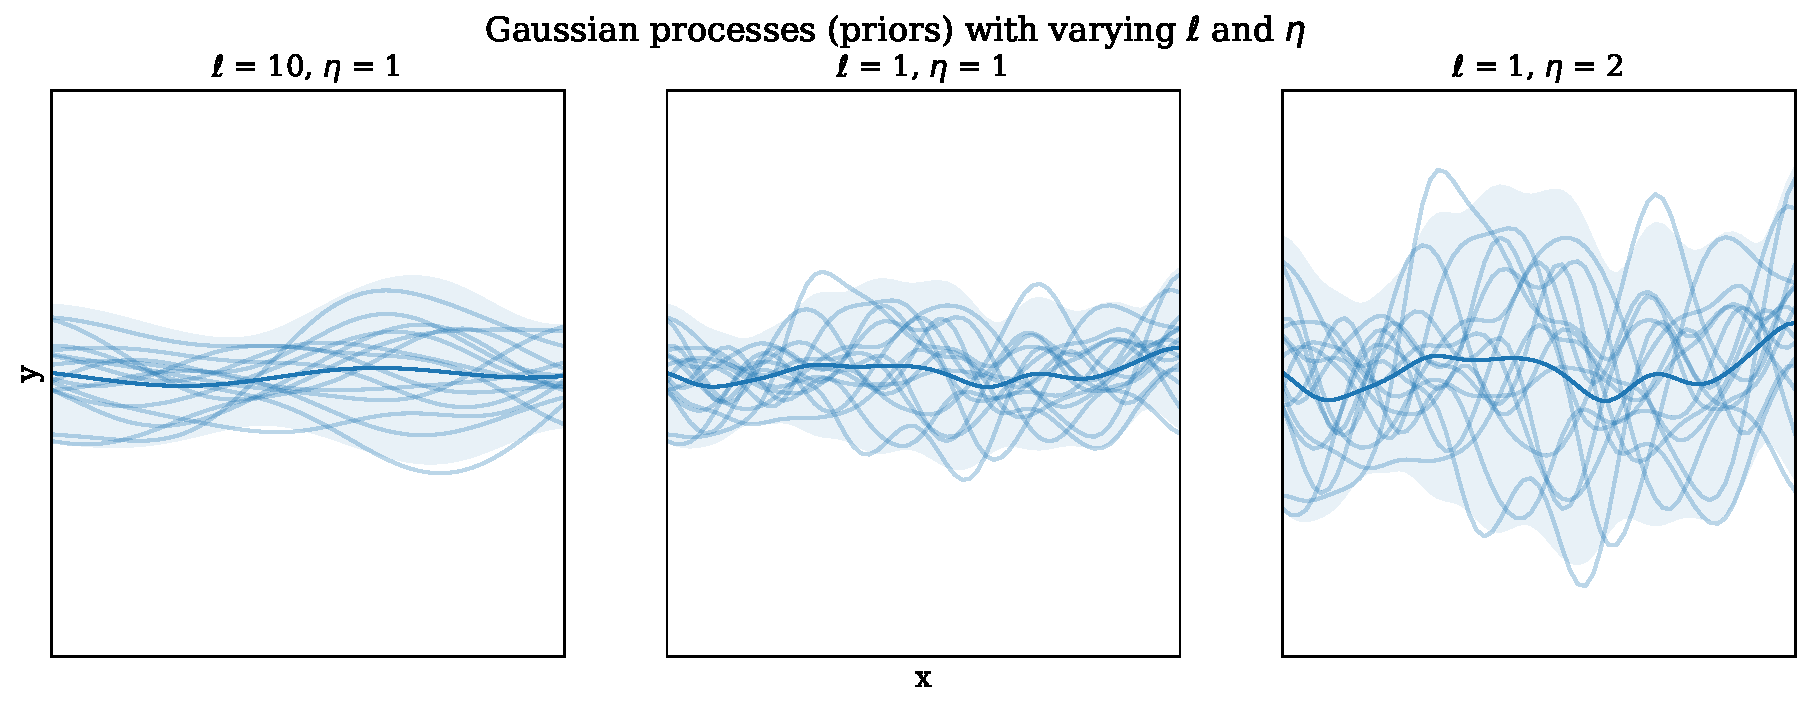
\includegraphics[scale=0.47]{GP_varying_hp.pdf}
    \caption{\footnotesize{15 functions drawn from three different GPs (priors) with different hyperparameters $\ell$ and $\eta$. All three GPs uses a squared exponential kernel function and a mean function = 0}}\label{GP_varying_hp}
\end{figure}

% Explaining the 1. example
The mean value across all 15 functions is the thick line and is denoted $\mu$. It is routinely used as the most-likelihood estimate of a functional form, and without any data it will default to the mean function \cite[3]{williams2006gaussian}. The volatility seen in \autoref{GP_varying_hp} is only due to the small number of samples drawn. The shaded area denotes two \emph{standard deviations} ($\sigma$) from the $\mu$ given the sample. Again, the volatility is due to the small sample number. Without any data introduced all functions given by the mean and covariance function are valid estimates. However, introducing data makes some functions more likely than others, effectively limiting the forms of the sampled functions. This is illustrated in \autoref{GP_toy_posterior} where the sampled functions now accommodate the data where it is available. Note that this Gaussian process is defined without any error term $\epsilon$.\par  

\begin{figure}[!htb]
	\centering
	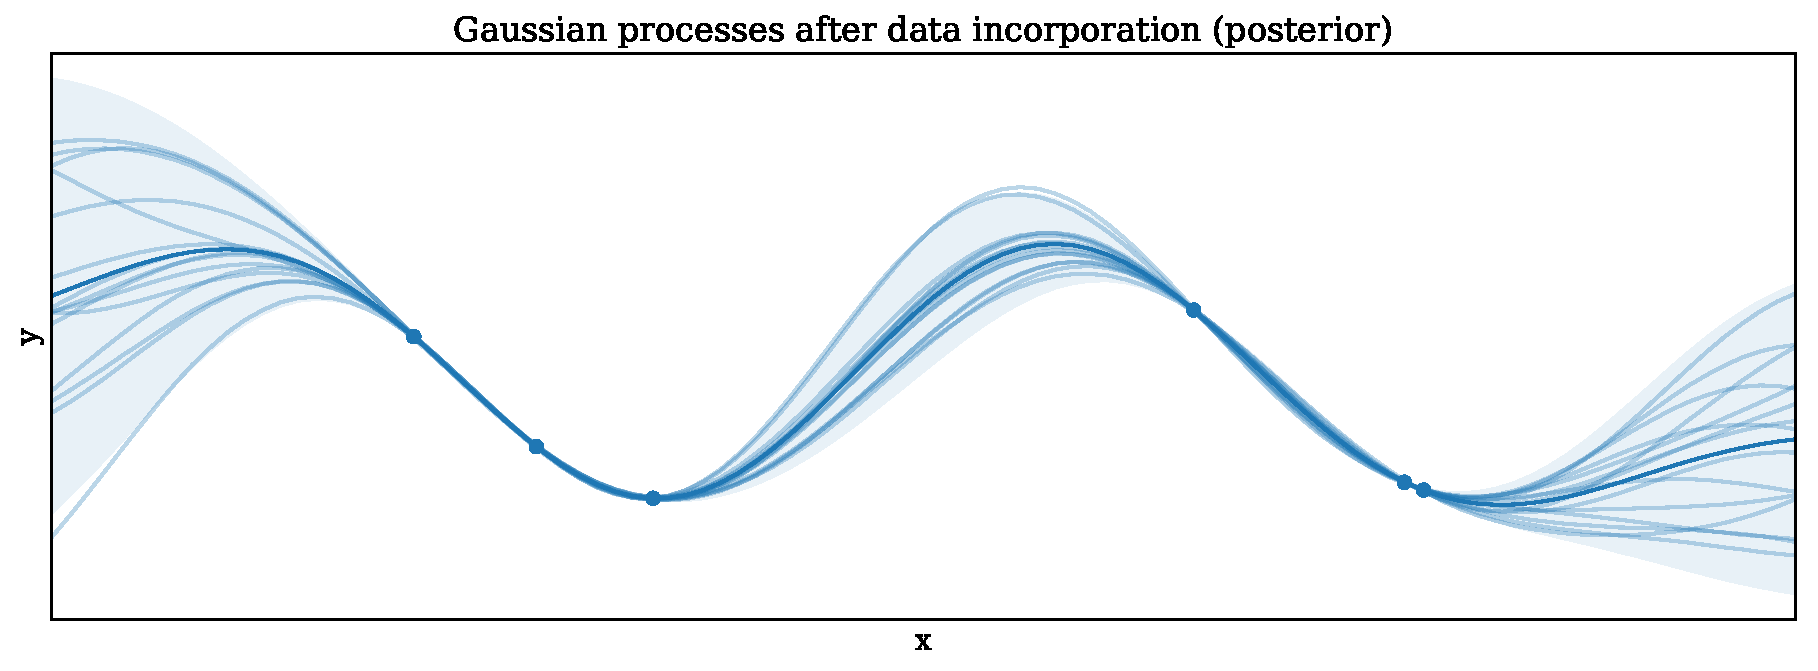
\includegraphics[scale=0.47]{GP_toy_posterior.pdf}
    \caption{\footnotesize{15 samples from A Gaussian process after the introduction of data. The points represents the data. The thick line is $\mu$ and the shaded area represents $\mu \pm 2\sigma$.}}\label{GP_toy_posterior}
\end{figure}

% Explaining the 2. example
Again, $\mu$ is the thick line and the shaded background represents $\mu \pm 2\sigma$. We see that uncertainty shrinks in regions illuminated by data, and grows the further we move away from data.\par

% concluding on examples
It should be clear from \autoref{GP_varying_hp} and \autoref{GP_toy_posterior} that if I were to determine the hyperparameter myself and omit an error term $\epsilon$, I could fit most smooth patterns with total precision. This would naturally lead to overfitting and furthermore, I would not have handled the issue of researchers guessing at functions rather than estimating them.\par

% Solution
Encouragingly, this can be amended rather elegantly. We included an error term $\epsilon$ to the Gaussian processes; which along with the hyperparameters $\ell$ and $\eta$, will be estimated through a framework which actively discourages overfitting. \cite[114-115]{williams2006gaussian}. Using the estimated error term and hyperparameters in tandem with our data will generate Gaussian processes which will fit to the general patterns of the data, but not overfit to noise.\par

% How this solution is don?
These estimates are obtained by maximizing the marginal likelihood of the given model \cite[114-115]{williams2006gaussian}. This, however, is a technical and non-trivial mathematical operation which I shall not explore further here\footnote{Curious readers should consult \cite{williams2006gaussian} section 5.4.1 for a complete overview and implementation of the operation.}.\par

% Exemple 3
A toy-example, emulating the subject of conflict magnitude, can be seen in \autoref{GP_toy_eks}. What we see here could be the development in three different conflict ridden geographic units from 1990 to 2018. Here $\ell$, $\eta$ and $\epsilon$ are estimated from the data. I have only included $\mu$, as the solid lines and the shaded areas represents an interval of two standard deviations given the underlying samples. Since we have observations for each year there is very little uncertainty regarding $\mu$ doing the observed years. We also see that the inclusion of epsilon lets the observations deviate from $\mu$, thereby discouraging overfitting to noise.\par

\begin{figure}[!htb]
	\centering
	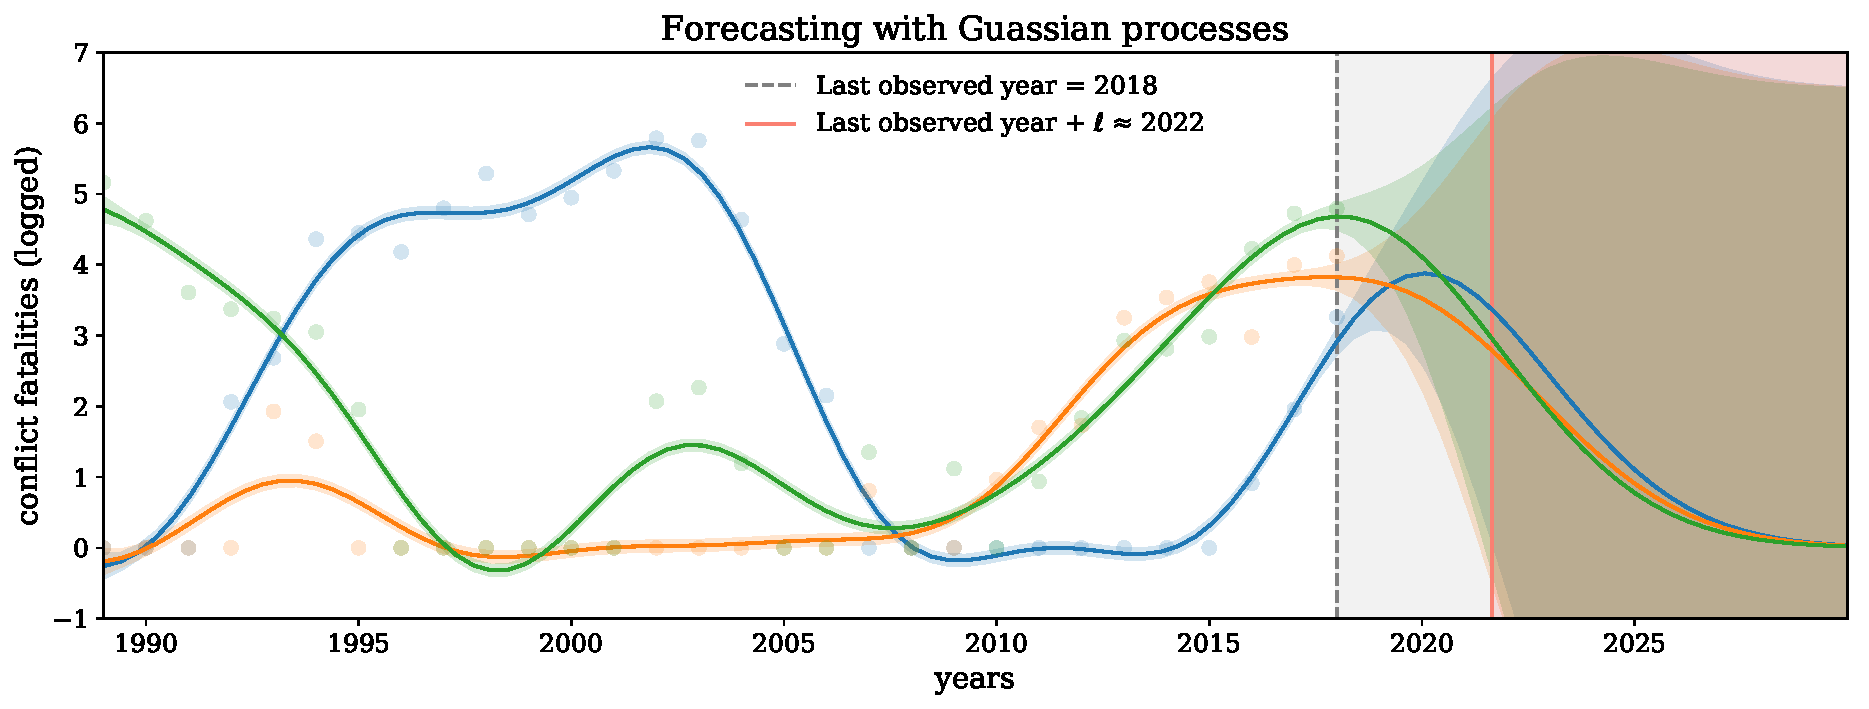
\includegraphics[scale=0.47]{GP_toy_eks.pdf}
    \caption{\footnotesize{Three (generated) time-lines of conflict ridden geographical locations. $\ell$ = 3.64, $\eta$ = 2.54, $\epsilon$ = 0.51}\label{GP_toy_eks}}
\end{figure}% you could make an ex with more noise.

In \autoref{GP_toy_eks} I have extrapolated 10 years ahead to illustrate how the two hyperparameters determine functional form of the function in the absence of data and how the mean function takes over as we venture into the unknown future. Crucially, I do not estimate a separate sets of hyperparameters for each of the three time-lines, but use the information from all three time-lines to estimate shared hyperparameters for all observations - so-called \emph{multi-task learning} \cite[115]{williams2006gaussian}.\par

% Patterns and non-zeroes
While I will use the same hyperparemater for all time lines in my implimentation, I will not use all time lines to estimate the hyperparameters. The reason is, that most time lines does not experience conflicts and as such does not tell us anything about conflict patterns. Including such "flat-lines" would yield a misleading estimate of $\ell$. The reason is that $\ell$ tells us how far we have to move on $x$ to see changes in $y$. Yet time lines with no conflicts have a consisting conflict magnitude ($y$) of zero no matter which year ($x$) we look at. As such the estimated $\ell$ would reflect that conflict magnitude is large constant across time \footnote{Indeed, preliminary tests showed that the models would often not converge at all, if I did not add a minimum of noise to the "flat lines".}. Naturally this is only the case for time lines experiencing no events and not time lines actually experiencing conflicts. To accommodate this issue the hyperparameters are only estimated using time lines with at least two years of conflicts (or later conflict exposure). While two might seem an arbitrary number, it stands to reason that you need at least two none-zero observations to constitute any kind of pattern.\par

% Your assumtions
As such, I assume that the broader patterns of conflict across time (and later space) are comparable across the observations\footnote{Using separated hyperparameters for all observations would be going too far and would mean that we do not think conflict patterns share any similarity across cases. Yet, less demanding assumptions could be made if we used a hierarchical structure which allowed the hyperparameters to be similar without being identical. Notably, that would entail a substantial increase in the computational resources needed.}. While the results from \cite{schutte2011diffusion} does support the use of the same covariance functions across all cases, it would be too bold to claim that the results conclusively supports the use of the same hyperparameters across cases. The validity of this assumptions should be further scrutinized in future endeavours. For now, however, this will do.\par

% Priors for hyper parameters
It should be briefly be noted that just as I have prior for my Gaussian processes, I also set priors for these hyper-parameters and the error term. More specifically I for the examples shown in \autoref{GP_toy_eks} instruct my program to search for these parameters within a pre-specified distribution as presented in equation \ref{eq:dist_ell}, \ref{eq:dist_eta} and \ref{eq:dist_epsilon}.

\[
\ell \sim \text{Gamma}(5,2)  \tag{8}  \label{eq:dist_ell}
\]

\[
\eta \sim \text{HalfCauchy}(2)  \tag{9}  \label{eq:dist_eta}
\]

\[
\epsilon \sim \text{HalfCauchy}(5)  \tag{10}  \label{eq:dist_epsilon}
\]


I will only use weakly regularizing priors here, which merely serves to discourage highly unrealistic values. These priors are easily overwhelmed by the patterns in the data, should the two not align. As such these prior only serves to increase computational efficiency and insure convergence \citep[35-36]{Mcelreath_2018}.\par 

% \begin{figure}[!htb]
% 	\centering
% 	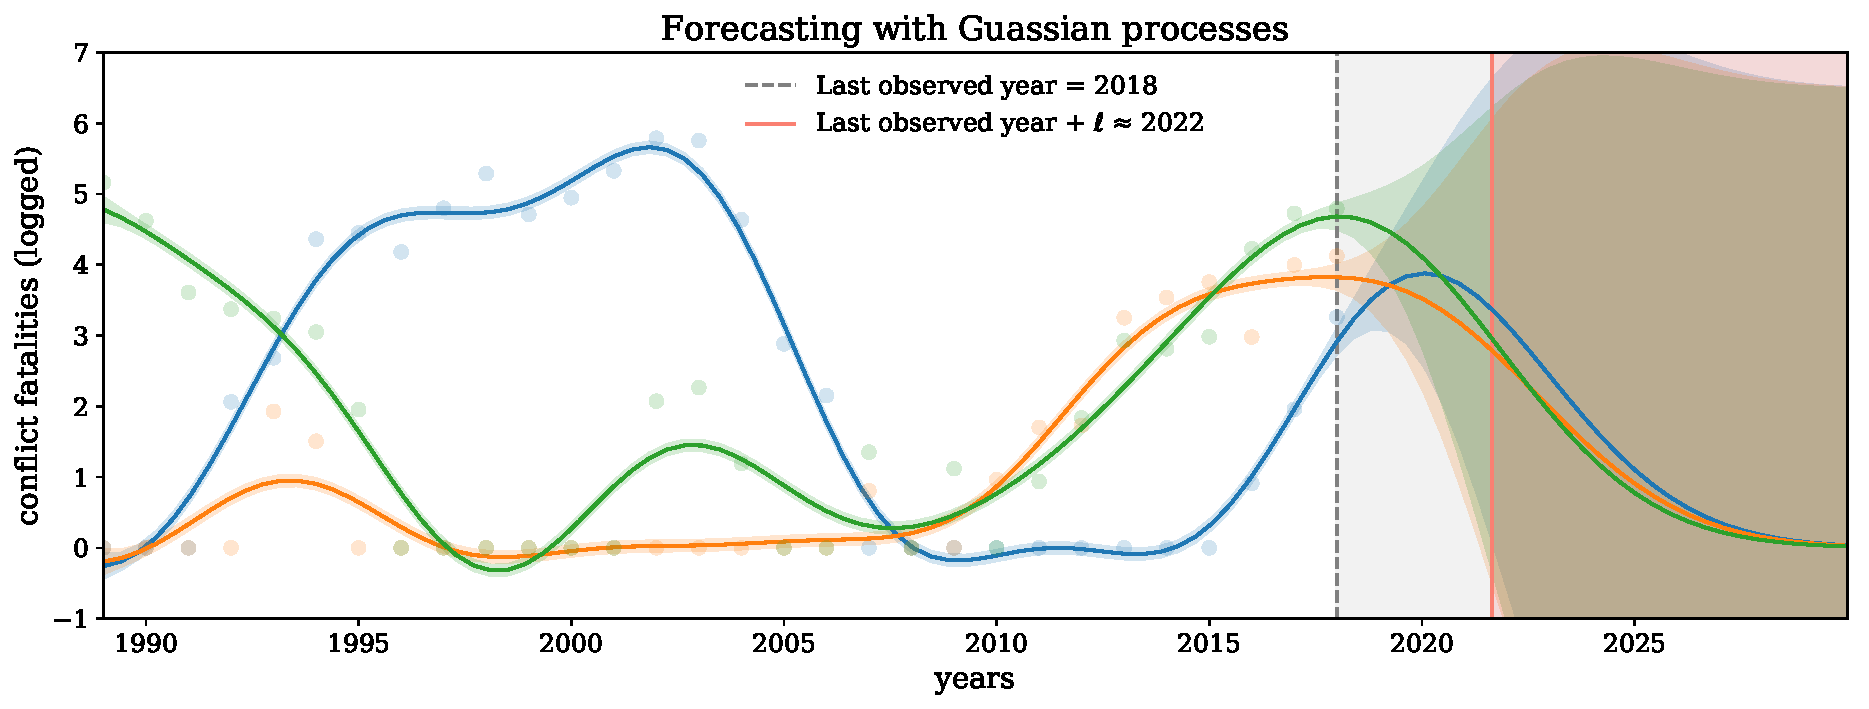
\includegraphics[scale=0.47]{GP_toy_eks.pdf}
%     \caption{\footnotesize{Three (generated) time-lines of conflict ridden geographical locations. $\ell$ = 3.64, $\eta$ = 2.54, $\epsilon$ = 0.51}\label{GP_toy_eks}}
% \end{figure}

% Concluding on the example:
In this toy example $\ell$ is estimated to be 3.64 with 95\% probability of being between 2.46 and 4.56. Thus, in this example it would be imprudent to extrapolate beyond year 2022 as indicated by the red line and shade in \autoref{GP_toy_eks}. Importantly, this hard limit is only a rule-of-thump, here given by the mean estimate of $\ell$. The specific uncertainty pertaining a given year should \textbf{always} be consulted in practice. In this example the uncertainty becomes extremely high after 2020. The mean of the three Gaussian processes are still valid estimates, but the prudent analyst should recognize that a "best guess" does not necessarily equal a "good guess". With this call for prudence in mind, \autoref{GP_toy_eks} does a good job of illustrating the potential of using Gaussian processes to model functions pertaining to the temporal pattern of conflict and how this framework allows easy extrapolation into future years.\par

% Changing to a spatial focus
To model the spatial pattern, I simply change the first dimension and include a second. That is instead of years, I use latitude and longitude. Here, the point is not to forecast into some unknown geographical space, but rather to let each observed cell incorporate information from all other cells in the data to estimate how exposed the given cell is to conflict. Naturally, the spatial and temporal patterns can also be combined into 3D space including two spatial and one temporal dimension, thus allowing for extrapolation of conflict exposure into future years.\par

% X_new
Having both estimated temporal patterns of conflict magnitude and conflict exposure, forecasting is simply a matter of introducing new future years; $x_{new}$ to the time lines. Now we simply generates Gaussian processes over these elongated time lines. The data of each specific time line in cohort with the covariance function and the estimated hyperparameters will guide how the function appears closest to the observed values, and the longer we stray from any observed value the more uncertainty will accumulate and the more influence the mean function will claim. 

% integration and differentiation:
Having actual functions extending into future years also allows for easy extrapolation of conflict \emph{slops} and \emph{acceleration} measures through differentiation and combined conflict \emph{mass} through integration. These are just derived function from $mu$ function estimated via Gaussian processor. As such, the values of these functions can also be used as individual features in a greater predictive framework.\par 
% should this be included in the criteria? 
%You should mention why it is theoriticly interesting nad potnetially usfulll

\[
\text{slope} = f'(x)   \tag{11}  \label{eq:slope}
\]

\[
\text{acceleration} = f''(x) \tag{12}  \label{eq:acc}
\]

\[
\text{mass} = F(x) \tag{13}  \label{eq:mass}
\]

% not actually function but values.
In practice I do not obtain a functional formula $f$ which I can work. Instead I simply get the values generated by the function $f$. As such equation \ref{eq:slope}, \ref{eq:acc} and \ref{eq:mass} denotes what I derive and extract, but not the actual computational operation used.\par

% er det her du skal sige noget interesant om dem eller? hvis du har teori tidlige så er det i hvert fald et godt sted at samle op.

%Another interesting potential of this approach is that we can also model a function as a combination of more functions; E.g. a short term trend and a long term trend \citep[505-510]{Gelman_2013}. In such a scenario the $\ell$ of a long term trend would be greater than the combined $\ell$ of both the short and the long term trend. It follows that the identifications of a long term trend would allow me to extrapolate further into the future with less uncertainty. Naturally, this is an opportunity which I shall take advantage of further on.\par

% Back to the criteria
Now, Revisiting the criteria I presented earlier, we see that Gaussian processes fulfill them all. In regards to the temporal pattern, they allow incorporation of information drawn from all past (included) years with decreasing influence \citep[410-419]{Mcelreath_2018}. Furthermore, the rate with which past years influence the forecastings is estimated through the data itself. These properties are the reason why Gaussian processes are often used to model functions over time \citep[13]{williams2006gaussian} Furthermore, no arbitrary "splines" or "knots" needs defining, which is one reason it has been recommend as a substitute to linear decay functions \cite[501]{Gelman_2013}. In regards to the spatial dimension, utilizing Gaussian Processes on a disaggregated geographical grid allows us to analyze and model spatial patterns at arbitrary high complexity levels only hampered by the resolution of the data and computational power available. We need not define the number of neighbours, since all observations are considered\footnote{That said, we could choose some appropriate subset to improve computation massively \citep{gelfand2016spatial} - but, regretfully, that is a project for an other time.}. Furthermore, we do not have to guess the deterioration rate of influence since this is estimated. Lastly, using Gaussian processes to model spatial diffusion, a given geographical cell will be influenced directly by the pattern and magnitudes of conflict around it, in a manner similar to the conflict patterns identified by \cite{schutte2011diffusion}. High magnitude will translate to higher influence, as will encirclement compared to tangency. Indeed, these properties are part of what compelled \cite{gelfand2016spatial} to declare the union of spatial data and Gaussian processes a "beautiful marriage" \citep[86]{gelfand2016spatial}.

%In regards to the spatial pattern this is ..... \cite{schutte2011diffusion} MEN! husk noget med friedman as-if... Du laver ikke noget kausal studio og kikker ikke på nogen mekanisme, men du mener stadig man skal gå efter at emulerer den data generende process i det omfang man har insigt, teori og empiri der muliggøre det. 

% But there are some problems... Below zero and space as degrees is more important then count...
Notably however, while I have illustrated the potential of the approach, it should also be clear from \autoref{GP_toy_posterior} that the framework presented here is somewhat misspecified. Since my base measure for conflict is conflict fatalities logged, one could argue that i should treat the data as count data. Since I will not be using the extrapolations directly as estimations of death tolls, getting fractions of death is not the problem. Instead the issue is that I will incidental estimate negative conflict magnitude and exposure. This will happen proceeding steep dives in temporal or spatial patterns.\par

% How cloud this be solved - and why it is not a problem
This could simply be handled by formulating the regression presented in equation \ref{eq:y} as a Poission regression. This is conceptually trivial, but unfortunately much more computational expensive and it introduces more complexity to an already complex endeavour. Somewhat encouragingly however, I ran initial tests which showed little to no difference when using a Poisson framework. The estimated $\mu$'s rarely dips below zero, and when they do it is only marginally. As such, I allow this misspicification to persist at the behest of simplicity and efficiency\footnote{A choice which is not unheard of  \cite[123]{williams2006gaussian}. A similar example can be found in \cite{Gelman_2013} chapter 21. Effectively, it is the same choice made every time a linear regression is used on count data such as death tolls, births, employment and indeed most data revolving around items or people.}.\par %your model is misspecified \cite[123]{williams2006gaussian}

% Next section
The next section will briefly present the theoretical underpinnings of the predictive framework which will transform the patterns estimated to actual predictions.\par 

%small $\ell$ less noice. Large $\ell$ more noice \cite[115]{williams2006gaussian}
%computational burdensome \citep[503]{Gelman_2013}


\subsection{The predictive framework}
% not the central endeavour!
% Her til er du kommet.

%[GP kunne altså godt bruges some pred i sin egen ret, men...]

% Whats going down here mate?
Naturally Gaussian processes can be used as predictive models in themselves; after all we forecast expected values into future years. However, to combined these forecasted values of conflict magnitude, conflict exposure and the derived measures of slops, accelerations and mass into unified predictions of conflict probability, we need an other tool. Indeed, Gaussian processes are often utilized as smaller components in larger models \citep[505]{Gelman_2013}. A predictive framework suitable for the challenge at hand have been presented in \cite{Maase}. Since the nature of this framework is not a prime concern in this thesis, I will not spend too much ink on this subject. A brief introduction, however, is in order. A more in-depth presentations can be found in tho original paper \citep[9-12]{Maase}.\par %While I here implement a number of improvements which I proposed in the conclusion of \cite{Maase} the setup is largely the same.
\par

% The specific elements
The framework consists of a number of individual elements best introduced in turn. first of all we need some algorithm capable of using the patterns extracted to estimation the probability of an event. We know that conflict are complicate phenomenons ridden with \emph{interactions} \citep[474]{cederman2017predicting}. Thus the predictive algorithm needs to be able to identify and generate such interactions. Furthermore, we know that conflicts are rare events. As such, the algorithm also needs to be pruned for handling rare events. For the sake of both policy recommendations and theoretical discussion it is also important that the algorithm is not a \emph{black box}; we most be able to asses which "decisions" facilitates the results \cite[476]{cederman2017predicting}. Secondly, even a algorithm pruned for rare events can have troubled handling the rarity of conflicts. As such I need tools which can mitigate some of the ills of imbalanced data. Final we need appropriate metrics for evaluating the potential of the endeavour as a whole. Metrics which again takes into account the rarity of the event gives us an honest evaluation of the framework potential. In the following subsections I show, in turn, how Extreme Gradient Boosting algorithm, Undersampling and the Precision-Recall curve can fulfill these roles.\par

%Bayesian Prior Correction ?

\subsubsection{Extreme Gradient Boosting}\label{xgboost}

% what is this shit?
The algorithm I use to estimate both the probability and magnitude of conflict is called \emph{Extreme Gradient Boosting} or simply \emph{xgboost} \citep{Chen_2016}. It is a machine learning algorithm somewhat more advanced then traditional regression analysis. That being said it here serves the same purpose. It can be constructed as a regressor to predict a number, similar to a linear regression or as a classifier to predict probabilities, similar to a logistic regression. In this thesis I will use it as a classifier to estimate the probability future conflicts in grid cells that constitutes the unit of analysis.\par

% What will you say about it?
However, this is also where the similarity between traditional regressions and xgboost cease. The xgboost algorithm is a rather new addition to the machine learning toolbox. From here it follows that it is a more complex construct than most political scientist have traditionally been exposed to. Luckily, one does not need a deep technical understanding of the algorithm to appreciate it's properties. As such, I shall refrain from getting into the nuts and bolts of the algorithm. Some base-intuition, however, will serve to qualify why this algorithm works remarkable well given the subject at hand. Particularly three characteristics deserves attention; it is a \emph{boosting} algorithm; it consists of \emph{regression trees}; and it is \emph{self-regularizing}.\par

% boosting:
Boosting entails aggregating a lot of weak classifiers to create a new single strong classifier. To this end, we evaluate the results from the weak classifiers and on basis of these results we distribute different weights across our observations. We now run a new batch of classifications but this time, the observations which was correctly predicted in the first round will carry lees weight while observations which was incorrectly predicted will carry more weight. This procedure is iterated until some predefined criteria is meet. Lastly, all classifiers are weighted according to the performance and used as a predictive ensemble to estimate the probability of some event \citep[338-339]{Friedman_2001}. This procedure ensures a continuing focus on "hard to classify" observations, and as such it is a particularly useful approach when working the rare events.\par

% !!!!!!!!!!!!!!
% regression tress - interactions er pointen!
Naturally we need to decide which weak classifiers to uses as the basis of our boosting. Xgboost utilizes regression trees\footnote{Which, strictly speaking are regressors and not a classifiers. Yet under the hood it is used as classifiers in the xgboost algorithm.} \citep[2]{Chen_2016}. A regression tree is a relative of the traditional decision tree. As such, the point is to partition our data according split-points which best sort our data according to some predefined target \citep[307]{Friedman_2001}. In the case at hand this would mean splitting grid cells experiencing conflict from cells that does not experience conflict. Yet, unlike decision trees, regression tree produces a continuous score, which can be converted into probabilities rather then the binary classifications of decision trees \citep[2]{Chen_2016}. The features and specific split points to be used are automatically found by identifying the splits that will minimize the sum of squares. We keep splitting partitions to increase prediction power until some predefined criteria is met - a criteria which is set in place to prevent overfitting \citep[307-308]{Friedman_2001}. Importantly this effectively means that the algorithm automatically identifies and generates the most salient interactions.\par
% !!!!!!!!!!!!!!

% self-regularizing
Naturally we need some way to set a appropriate criteria for when the splitting should stop. Conventionally this criteria is some specified minimum size of the partition to be split \citep[308]{Friedman_2001}. However, xgboost employs more systematic self-regularizing. To combat overfitting more effectively the regression tress used in the Xgboost algorithm penalizes overly complicated tress. Specificity, when the algorithm are to evaluate whether to further split a given partition, the potential information gain is down-weighted corresponding to the complexity induced by such split \cite[4-7]{Chen_2016}. Thus, the regression trees used in the boosting effort searches for relevant patterns in the data, but automatically stops before overfitting commence.\par

% Feature imp.
Finally, since the xgboost algorithm is based on regression trees, we can readily asses which splits generated most prediction power, and thus which features are most \emph{important} in regards to the combined prediction effort. While this tells us nothing about causation, it is still highly relevant for future prediction frameworks; for theoretical debates pertaining to explanations; and for concrete policy recommendations.\par

% Bridge - good for undersampling but no good enough
Naturally, this is a very superficial introduction to the xgboost algorithm; never-the-less it serves to illustrate why this algorithm is especially suited for the endeavour at hand. The boosting element makes the algorithm suitable for rare events and the fact that is is based on regressions tress both allows for automatic generation of interactions and for assessment of feature importance. Importantly the specific trees used in this algorithm are  self-regularizing thus discouraging overfitting. As such it is a very suitable framework indeed. Yet we can still do more. Particular in regards to the imbalance of the data. The next section will introduce a number of \emph{undersampling} techniques which I impliment to further tackle the rarity of conflict events.\par 

\subsubsection{Undersampling}
% Her til er du nået +++++++++++++++++++++++++++++++++++++++++++++++++++++++++++++++++++++
%\todo[inline]{IN PROGRESS}

% what is Imbalance?
%"Specifically, this form of imbalance is referred to as a between-class imbalance; not uncommon are between class imbalances on the order of 100:1, 1,000:1, and 10,000:1, where in each case, one class severely outrepresents another [4], [5], [6]. [...]Imbalances of this form are commonly referred to as intrinsic , i.e., the imbalance is a direct result of the nature of the dataspace" \citep[1264]{He_2008}

% what is undersampling?
When our data is highly imbalanced, the predictive algorithm used will often favor the classification of the majority class. In my case this would mean the the framework focused more predicting the absence of conflict rather then actual conflict. Using a boosting algorithm such as xgboost does a good job of ameliorating this problem - but we can do more. A simple and logical solutions is simply to undersample the majority class. As such in our test set we drop a portion of non-events to even the ratio between events and non-events. This is called undersampling \citep[1266-1267]{He_2008}. 

% What do you do? - 
Specifically I combine two procedures \emph{case-cohort sampling} and \emph{informed undersampling}. Case-cohort implies, that when I train my model I use all available events present in the train set and a randomly drawn subset - equally sized - of non-events also from the train set  \citep[142]{King_Zeng_2001}. This procedure is usually justified by arguing that more information is stored in the events, than in non-events \cite[139]{King_Zeng_2001}. While this may be true, I still discard a lot of potential information this way. To amend this information-waste I embed this appraoch in a variant of informed undersampling. Instead of just using one model with one random subset of non-events I use an large \emph{ensemble} of models each using a new random subset of non-events \cite[1267]{He_2008}. Specifically I run the xgboost algorithm 1000 times; each time with the full set of (train) events and a randomly drawn subset of (train) non-events. As such I am effectively estimate a distribution of the conflict probabilities for each cell taken advantage of all the information in events and non-events alike. Naturally I can then use the mean of these distributions as a maximun likelyhood point estimate for the actual probability. Furthermore, given that I can also asses the variance of these distributions, I am also able to infer how certain I am of this point estimate.\par 

% Introducing the Baysian correction
One issue with this undersampling approach is, that the specific probabilities produced will be somewhat inflated. After all each of the 1000 models run thinks that conflict is much more common then is actually the case. This, however, can easily be amended using a \emph{Bayesian prior correction} akin to what is presented in \cite{King_Zeng_2001, king_zeng_2001b} and implimented in \cite{Goldstone_2010}. I use the overall probability of conflict in the last observe year in my train set: 2012. This is simply the ratio between events and non-event. I denote the share of events $Pr(E_{2012})$ and the share of non-events $Pr(NE_{2012})$. Then, denoting the the estimated probabilities of an event in a specific cell at a specific year $Pr(E_{estimated})$; the corresponding estimated probabilities of a non-event $Pr(NE_{estimated})$; and the corrected probabilities of events as $Pr(E_{corrected})$ the correction can be expressed as follows:

\[
Pr(E_{corrected}) = \frac{Pr(E_{estimated}) \times Pr(E_{2012})}{Pr(E_{estimated}) \times Pr(E_{2012})+Pr(NE_{estimated} \times Pr(NE_{2012})} \tag{14} \label{eq:bayesC}
\]

% concluding on it:
This correction ensues that the probabilities estimated matches the "empirical" probability of conflict in the real world. Notably however, this does not make my framework more or less precise. The reason is that, if we want to turn our estimated probabilities into actually classifications we still need to set some probability threshold splitting our estimates dichotomous into predicted events and predicted non-events. This threshold is normally set at 0.50, but this threshold is arbitrary as any other number would be \citep[890-891]{weidmann_ward_2010predicting}. Indeed, any such threshold should always be chosen with the specific subject in mind \citep[194]{Goldstone_2010}. As such, since the correction does not change the relative difference between the estimated probabilities, I could get the same binary classification both with and with out the Bayesian correction if I just used two different thresholds. One high threshold for the uncorrected estimates, and one lower threshold for the corrected estimates. However, the probabilities obtained after the correction are still preferable since they incorporate information regarding actually conflict propensity in the real world. As such they correctly conforms to how we usually understands probabilities. This is crucially since I do not recommend using binary classification for decision making purposes. The actual probabilities holds much more information and should always be consulted.\par

%bridge
Together, the xgboost algorithm and the undersampling approach taken, does a good job of priming the framework for rare events. However, both these efforts does so trough the model training; the test data we feed our model will still be imbalanced. We cannot undersample this data since it role is to emulating an unknown future. Undersampling it would imply that we already know which cell we be events and which will be non-events. The consequence of imbalanced test data is that conventional evaluation matrices tend to asses such models too favorable \citep[1264]{He_2008}. The next section will introduces the evaluations matrices which I use for this project, and qualify why these are appropriate for evaluating unbalanced data.\par


\subsection{Evaluating Predictions}
%\todo[inline]{TODO: Precision-recall curve}
%Samme som sidst, men må ikke fremstå som plagiat... Og denne gang skal du også have AUC med for at kunne sammenligne med andre efforts.

% The two different estimation efforts.
For the construction of my framework I use two layers of estimation. First, I use Gaussian processes to estimate the pattern of conflict magnitude and conflict exposure. Secondly, having extrapolated these patterns into future years and derived the corresponding slope, acceleration and mass, I use these patterns as features in my final predictive framework which is based on the xgboost algorithm and various undersampling methods. I will then use this final predictive framework to asses to probability of future conflicts. Naturally to asses whether I truly captured any salient conflict patterns with the Gaussian processes I most evaluate how well the final predictive framework performance; how good my predictions actually are.\par

% Out-of-sample prediction
Given the predictive scope of my project I employ out-of-sample prediction to evaluate the performance of my approach. Out-of-sample-prediction is implemented by using a subset of my data to train my predictive framework and an other subset to test the framework. Given that my goal is practical forecastings I use the last five years of my data as testset. As such, to construct the final predictive framework I use a target $y_{train}$ and the features I have constructed via Gaussian processes $X_{train}$. When I want to create prediction, I introduce $X_{test}$ to my predictive framework to produce out-of-sample predictions $y_{pred}$. These prediction can the be evaluated against the empirical observations $y_{test}$.\par

% What are yo gonna do?
Now, having my predictions $y_{pred}$, and the empirical observations $y_{test}$ I need some metric which can captures how well $y_{pred}$ fits $y_{test}$. There are a plethora such metrics available. The metric I will primarily use is the \emph{Precision-recall} curve and the three related metrics \emph{recall}, \emph{precision} and \emph{average precision}. However, to put these metrics into perspectives I will also introduce the metrics \emph{accuracy} and the \emph{Receiver Operating Characteristic} curve along with the corresponding metric the \emph{Area Under the Curve} (AUC) score.\par

% Criteria for a good measure/why no hard threshold.
Naturally the metrics used most fit the challenge at hand; not least the fact that I am dealing with imbalanced data. Furthermore, many metrics require that I set some hard threshold partitioning my predictions into predicted events and predicted non-events. My framework, however, does not produce binary results but probabilities. As such $y_{test}$ might by binary  - either $0$ or $1$ - but $y_{pred}$ can take any value between $0$ and $1$. These probabilities are in themselves far more informative than a simple binary classification. As such the metrics I use should not depend on the formulation of some arbitrary hard threshold.\par 

% Introducing Acc and error/ the problem the Acc and error
The most commonly know metric for classification efforts is \emph{accuracy}\footnote{or the inverse error-rate}. Accuracy simply denotes the ration of correctly predicted observations. As such accuracy is easy to interpret and intuitively appalling. However, there are two problems. First of all the measure requires that we choose a hard threshold. Secondly when the data is imbalanced we can achieve a rather high accuracy be just predicting in favor of the majority class every time. If conflict only happen 5\% of the time we can get an accuracy of 95\% by simply predicting that conflict never happens. As such accuracy is not very suited for imbalanced data \citep[1264]{He_2008}, and thus while this is the best known measure, I will not be using this metric going forward.\par


% Introducing AUC (and TO/TN/FN/FP)
The metric most commonly chosen to avoid the problems of accuracy is the ROC curve and the summarizing measure the AUC scores \citep[1277-1278]{He_2008}. The ROC curve circumvents the issue of a hard threshold by evaluating each possible threshold. Specificity the ROC curve denotes the tradeoff between the \emph{true positive rate} ($TP_{rate}$) and the \emph{false positive rate} ($FP_{rate}$) by plotting the $TP_{rate}$ over the $FP_{rate}$. This curve can then be interpreted visually or summarized by the area under it; the AUC \citep[1277-1278]{He_2008}. Denoting the actual number of negatives $N_C$ and the actual number of positives $P_C$, the rates can be expressed by equation \ref{eq:TPFP}.\par

\[
TP_{rate} = \frac{TP}{P_C};\quad FP_{rate}=\frac{FP}{N_C} \tag{15} \label{eq:TPFP}
\]

% concluding on AUC
As such the ROC curve does not require us to specific a hard threshold and it illustrates clearly the trade-of between true positives and false positives at all possible thresholds. Given these attribute it has been widely used in conflict studies \citep[14]{chadefaux2017conflict}, and even been coined as the "gold-standard" in this field \citep[366]{perry_2013}. 

% The problem with AUC in imbalanced problems - and why it is still here
However, while better suited for imbalanced data, than accuracy, the ROC curve and AUC score tends to judge model-performance on highly imbalanced data too favorable \citep[1278]{He_2008}. Looking at equation \ref{eq:TPFP} it is clear that if we can increase $N_C$ whit out increasing the $FP$ rate we will get a better score. As such, including Antarctica would probably improve my results substantially. Antarctica would constitutes a large number of non-events ($N_C$) and given my focus on past conflict patterns my framework would never produce a false positive ($FP$) here, leading to a lower false positive rate ($FP_{rate}$).\par

% Why is it still here
Despite this weakness I will still report the AUC score. The simple reason is convention. the ROC curve and AUC score is a point of reference for most political scientist working with advance quantitative methodes and including such measure will make it easier to compare my project with past efforts. That being said we should move on to more appropriate metrics better suited for highly imbalanced data. As such my main focus will be on the PR curve.\par

% Intorducing Precision, Recall, PR-curve and average precision.
The PR curve shares many similarities with the ROC curve. It also denotes the trade off between two measure. Specifically \emph{recall} and \emph{precision}. Denoting true positives $TP$, false positive $FP$, true negatives $TN$ and false negative $FN$, recall and
precision can be expressed as in equation \ref{eq:recall/precision}.\par% and \autoref{eq:precision}.\par 

\[
precision = \frac{TP}{TP+FP}; \quad recall = \frac{TP}{TP+FN} \tag{16} \label{eq:recall/precision}
\]

% \[
% recall = \frac{TP}{TP+FN} \tag{17} \label{eq:precision}
% \]

% int the equations:
As such, precision denotes how many of my predicted events turn out to actually be events, while recall denotes how many of all actual events I captured with my predictions. These two measure are in themselves valid metric and they are both highly relevant when dealing with imbalanced data. However, since these metrics relies on components such as $TP$'s, $FP$'s, $TN$'s and $FN$'s both metrics requires a hard thresholds. Combining them in a curve for all possible thresholds eliminates the need for any hard threshold and concurrently summarizes both metrics neatly \citep[1287]{He_2008}.\par

% Average precision
The PR curve can be interpreted visually and also be summarized be a single measure call average precision ($AP$). This summarizing metrics denotes a weighted mean of precision at each possible threshold. The weighting is the increase in recall from the previous threshold. Denoting recall $R$, precision $P$, and the different thresholds as $n$ the AP score can be expressed as seen in equation \ref{eq:ap}.\par

\[
AP = \sum_n (R_n-R_{n-1})P_n \tag{17} \label{eq:ap}
\]

% compared to AUC?
The AP score have a number of similarities with AUC and can be thought of as as the area under the PR curve  \citep[349-350]{su2015relationship}. The key difference is that AP places more emphasis identifying high probability events then identifying low probability events \citep[350]{su2015relationship}. The interpretation also differs from AUC. An AUC score of 0.5 denotes a classifier which is no better then random. This is not the case with AP where 0.5 can be a decent score depending on the context \citep[350-351]{su2015relationship}. As such AP is a good summarizing measure for judging and comparing the predictive performance of models on imbalanced data without setting a hard threshold. I will use it both to compare my results with the results presented in \cite{Maase} and to show how the predictive power of my framework changes as I move further into the future.\par

% The downside and the solution
The downside of AP is, that it is not not especial interpretable on a substantive level. As such, to best present the potential of my framework in substantial terms I will use the AP score in cohort with recall and precision at various thresholds. In the same manner I will also us the components $TP$, $FP$, $FN$ and $TN$ for visualizations. This will naturally demand that I set some hard threshold. I use a threshold which generates a number of predicted events which roughly matches the number of actually events in the last observed year: 2012. This threshold is as arbitrary as any other hard threshold chosen, but it serves well to create interpretable visualizations. In cohort these measures will ensue both honest evaluation and interpretability of my framework.\par % you could also map with different thresholds....

% Bridge
Having presented the methods which I will use to construct my predictive framework, I will now move on to present the specific data which I use. As such the next section serves as the last primer before I present the implementation and the results.\par

\section{The Chosen Data}\label{data}% you have the essence in the introduction...

% Whats go happen here mate?
In this paper I use two data sources; the Upssala Conflict Data Program(UCDP) \citep{Sundberg_2013, Croicu_Sundberg_2017} provides all substantial data used, while the spatial grid which divides the world into cells is borrowed from the PRIO grid database \citep{Tollefsen_2012}. I will present each sources in turn below.\par

\subsection{The PRIO grid}

%What PRIO DATAbase?
The PRIO grid database holds large roster of features denoting wealth, mountains, ethnic discrimination and much more, partitioned at sub-national level. In this paper I do not use any of these features. I only uses the geographical base-grid which the database provides. Not only does this save my the hassle of constructing my own grid, it also allows for PRIO grid features or data prime for the PRIO grid to be easily Incorporated in future endeavours. Science is a cumulative effort after all.\par 

% What the PRIO gird
The PRIO grid is a global grid divided the world - excluding Greenland and Antarctica - into grid cells of $0.5 \times 0.5$ decimal degrees, which corresponds to roughly $50km\times50km$ at the equator \citep[367]{Tollefsen_2012}. It is constructed as geo-spatial (vector) data and primed for collaboration with the UCDP data. As such merging and handling these two data source is a trivial task. However, do to computational limitation I have chosen only to use a subset of the full globe. This subset is presented in \autoref{map_2017}.\par

% er tallen serif?
\begin{figure}[!htb]
	\centering
	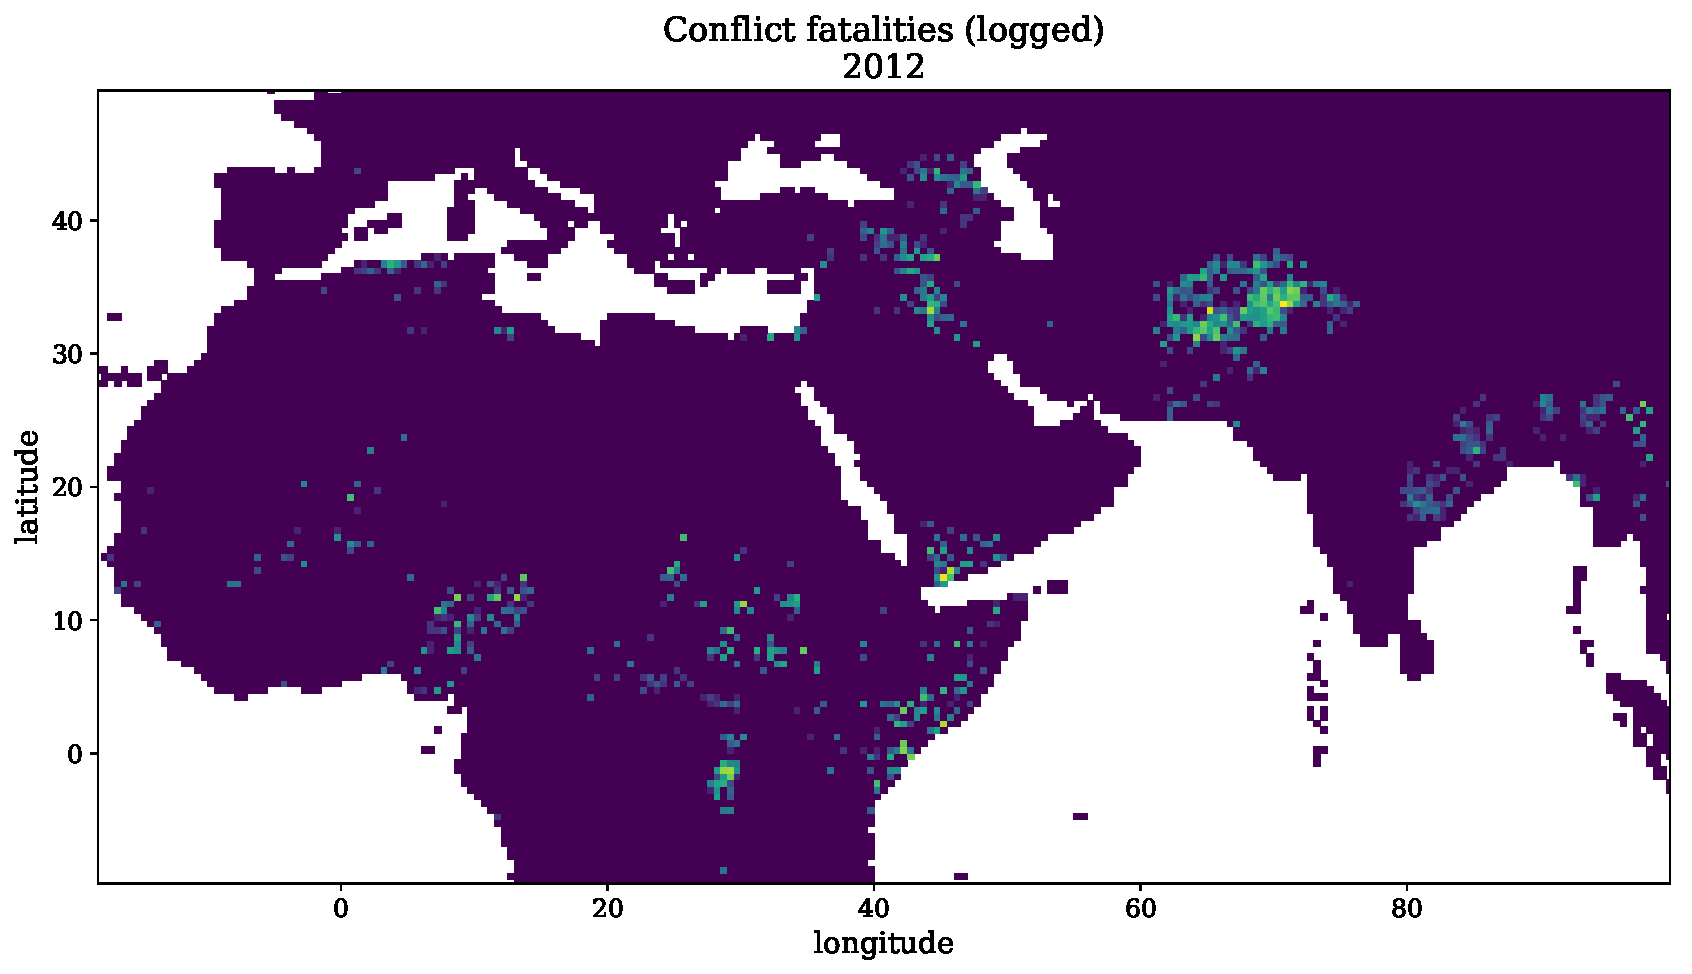
\includegraphics[scale=0.5]{log_best_2012_samples.pdf}
    \caption{\footnotesize{Conflict fatalities (logged) from 2017 according to UCDP aggregated at the level of PRIO grid cells.}}\label{map_2017}
\end{figure}

%interpreate the map
In \autoref{map_2017} I have plotted all conflict fatalities (logged) classified by UCDP in 2017 aggregated at PRIO grid cell level in the chosen subset. While the exact boarders of the subset are rather arbitrary\footnote{north: 50*, south: -10*, east: 100*, west -20*}, I have aimed to encompass as many conflicts as possible, across the surveyed timespan, encompassed in one continues geographic area. As such, the subset encompasses more or less conflict-prone regions such as Balkan, Caucasus, Syrian, Iraq, Yemen, Palestine, Rwanda, Kashmir, Afghanistan, Nepal, Aceh, Sri Lanka, Rwanda, Mali, Nigeria and many more. With a more computationally power the rest of the globe could be readily Incorporated into my framework.\par

% selecting on the dependable
Naturally, this is selection on the dependable variable, and as such it will lead to bias in any estimation effort \citep[129-130]{king1994designing}. However, I have no traditional parameters to estimate and no claim of effect or causality to make. Thus, since accurate prediction as the goal, selection on the dependable variable is less of a problem then with traditional estimation efforts. Furthermore, any ills could easily be handled through yet another Bayesian corrections \citep[627-628]{King_Zeng_2001}. That being said, it would still be imprudent to extrapolate any insights I produce - such as the estimated hyper parameters - beyond the geographical scope of the project. Correspondingly the probabilities I produce should be seen as conditional of the geographical subset under scrutiny.\par


% This precaution, however, is not enough. On one hand selecting a geographic area with relatively many conflicts is a way to battle the imbalance of the data. Indeed " the real information in the data lies much more with the ones than the zeros" \citep[139]{king_zeng_2001b}. One the other hand, however, our model will "believe" that conflict is much more common then it is. This is already a problem given the effort to battle to imbalance of the data as presented in \autoref{imbalanced} and thus the remedy the same already introduced; a baysian correction similar to that presented in \cite{King_Zeng_2001} and implemented in \cite{Goldstone_2010}.\par 
% Er det den ritige henvising?

% Having present, the context, the challenge, the tools and the data which I use, the next section while present the implementation.\par
% Bridge
With this call for prudence I now introduce the substantial data which I will use to capture conflict magnitude and exposure.\par

\subsection{The UCDP data}

%\todo[inline]{Her du skal sige hvilket år der er test og hvilke der er train}


% Two layers; many different y and x's -> how to keep up?


% What is the UCDP?
My framework consists of two layers of estimations. First I estimate the patterns of conflict magnitude and conflict exposure. Then I use these estimated patterns to estimate the probability of conflict in a cell at some future year. The only data I need for these two endeavours is data pertaining directly to the history of conflict patterns. For this I use the \emph{Uppsala Conflict Data Program} (UCDP) \citep{Sundberg_2013, Croicu_Sundberg_2017}. Specifically I utilize the UCDP Georeferenced Event Dataset (GED) Global version 18.1 \citep{UCDP_2017}. The data contains records of conflict fatalities and the corresponding coordinates and dates. I aggregate this data to yearly fatalities and utilize data from 1989 through 2017\footnote{For a smaller less detailed feature space data is available going back through 1975}.\par 

% How is conflict fatalities defined
I define conflict fatalities using the very minimal definition from UCDP. They included in their data all fatalities where "armed force was used by an organized actor against another organized actor, or against civilians, resulting in at least 1 direct death at a specific location and a specific date”.\cite[9]{Croicu_Sundberg_2017}\footnote{Se definitions regarding "armed force" and "organized actor" page 10 and forth of \cite{Croicu_Sundberg_2017}.}\par 

% onlys intra
Since I limit my project to intra-state conflict, I only included estimates from incidents which do not include two different nations as the organized actors. What is left is all conflict fatalities induced by internal conflicts, civil strife and terror.\par

% what do you uses?
There are a number of interesting features included in the UCDP data. I only use the feature \emph{best}. This feature is defined as: "The best (most likely) estimate of total fatalities resulting from an event." \cite[7]{Croicu_Sundberg_2017}. To get my raw measure of conflict magnitude, used as a target in my pattern estimation efforts, I take the log of this measure.\par

\[
\text{conflict magnitude} = log(\text{conflict fatalities}) \tag{18} \label{eq:cm}
\]

% Why log?
The log-transformation is warranted since the data is highly skewed; most cells experience no conflict fatalities most of the time, while a very few cells experience a lot of conflict fatalities. Furthermore a logged transformation mitigates the challenges of extreme outlets such as Rwanda 1994. For the final predictive effort I construct a binary target simply denoting whether or not a given cell is experiencing any conflict at all.\par

% Different y's and x'x
This measurement, conflict magnitude, aggregated at the yearly level and distributed across the Prio grid is the basis for my whole framework. In the first layer it will by the target $y_{cm}$ when I estimate the pattern of conflict magnitude, while years will constitute the single feature $x_{year}$. When I estimate the static conflict exposure for each year it will also be the target $y_{cm}$ while longitude and latitude will be the features $X_{ll}$. In the second layer, a binary transformation of conflict magnitude will constitute the target $y_{binary}$ when I estimate the probability of conflict using the last predictive frame work , while the features will be the eight features derive in the first estimation layer will constitute the features $X_{patterns}$.\par

% what will be test and what will be train?
Giving that I am producing forecasting I use the last five years of my data, 2013 through 2017 as test set, and all other years - from 1989 through 2012 - as my train set.  As such, I use a ratio of roughly 20\% for the test set, which is rather conventional \citep{Friedman_2001, Ward_Greenhill_Bakke_2010}.\par

% MEN SKAL DET HER ST HERÅ? +++++++++++++++++++++++++++++++++++++++++++++++++++++++++++++++
% Illustratively, in \cite{Maase} I used the PRIO grid database to obtain the structural features at a disaggregated sub-national level \citep{Tollefsen_2012}. This database holds a plethora of interesting features at disaggregated sub-national level, most with some relevance in regards to conflict prediction.. The database is indeed impressive, yet the challenge of using this data - and indeed most data like it - for forecasting, is that it takes researchers a lot of time to collected, process and make accessible. Both for the researches at PRIO and the researches responsible at each original source. At the time of writing - 2019 - the most up-to-date features have the last entry at 2015, while some have last entry at 2010; a five to ten year lag if I want to predict the conflict zones of 2020. This is less than optimal to say the least. Even if one where to bypass the Prio Grid database and go directly to the different original sources of data, much would still be lagging, and it would be a huge burden to collect, clean and merge these various data sources.\par

% Conversely, for data relating to the spatial/temporal pattern of conflict we only need one data source; on pertaining to when and where conflict has taken place in the past, e.g. the UCDP. At the time of writing the last entry in the UCDP is from 2017, and the given past history the entry for 2018 is due sometime doing the first half of 2019. A clear advantage compared the the PRIO gird database. As such, I might not be able to use data from 2019 to predict events in 2020, but I would be able to use data from 2018 to predict events in 2020 and onwards; a manageable two year lag.\par
% +++++++++++++++++++++++++++++++++++++++++++++++++++++++++++++++++++++++++++++++++++++++++++++

%bridge 
Having presented the context of my project, the tools I employ and the data used, I now move on the actual creation of my framework.\par

%In the next section I will estimate and extraplote the patterns of conflict magnitude and conflcit exposure 

\section{Compiling the framework}% Better name?

% What is gonna happen here?
The following section is divided into two subsections corresponding to the two layers of estimation I employ. Firstly, I estimate the temporal and spatial patterns of conflict using my test set and Gaussian processes. These patterns will then be extrapolated into future years corresponding to those of the test set. From these elongated times lines I will then derive the corresponding slope and acceleration pertaining to each year, along with the total conflict mass inhabiting each time line. This yields eight features. Secondly, using xgboost and undersampling, these eight features will be combined in my final predictive framework to estimate the probabilities of conflict in each individual grid cell given the test years from 2013 through 2017. An overview of the two layers of estimations is presented in \autoref{overview} - for brevity I omit the extrapolation efforts in the table.\par

% HP table
\begin{table}[!htb]
\begin{center}
\centering
% 	\begin{tabular}{l*{4}{c}}
	\begin{tabular}{m{1cm} m{1.8cm} m{6cm} m{0.2cm} m{4cm}}
	%\hline
	\textbf{Estimations}
	\\Overveiw\\
	\hline
    & Target $(y)$                            &  Features $(x/X)$                    && Estimate $(\tilde{y})$  \\
	\hline
	\\
	\thead{\\}                  &$y_{cm}$                                & $x_{year}$                           && $\tilde{y}_{cm} = f_{cm}(x_{year}) + \epsilon_{cm}$        \\
    \thead{First\\layer}        &$y_{cm}$                                & $x_{long}$, $x_{lat}$: $X_{ll}$       && $\tilde{y}_{sce} = f_{sce}(X_{ll}) + \epsilon_{sce}$           \\
    \thead{\\}                  &$f_{sce}(X_{ll})$                       & $x_{year}$                           && $\tilde{y}_{dce} = f_{dce}(x_{year}) + \epsilon_{dce}$        \\
    \\
    \hline
    \\
    \thead{Second\\layer}       &$y_{cmBinary}$                           &  $f_{cm}(x_{year})$, $f'_{cm}(x_{year})$, $f''_{cm}(x_{year})$, $F_{cm}(x_{year})$, $f_{dce}(x_{year})$, $f'_{dce}(x_{year})$, $f''_{dce}(x_{year})$, $F_{dce}(x_{year})$ : $X_{patterns}$     &&$\tilde{y}_{prob}$ \\
    \\
    \hline
	\end{tabular}
\end{center}
\caption{\footnotesize{Targets, features and estimates pertaining to the various estimation efforts in the two next sections.}}\label{overview}
\end{table} 

% Math will be in the appendix
% or? 

% Afterwards
In the proceeding section I will then present the results and evaluate the performance of my approach. That is; assessing whether or not I have actually identified and extracted conflict patterns which can be used to predict the time and place of future conflicts. 
%\todo[inline]{Why the two baseline conflict exposure and conflict magnitude}
%\todo[inline]{Why the there derived measures: slope, accelaration and mass?}

\subsection{First layer: Patterns as features}
%[HERTIL ER DU KOMMET!!!]+++++++++++++++++++++++++++++++++++++++++++++++++++++++++++++++++++++++++++++++++++++++++++++++++++

%First I will estimate the temporal and spatial patterns of conflict in each grid cell at all years in included in the train set using Gaussian processes. These patterns will then be extrapolated into future years corresponding to those of the test set. From these elongated times lines I will then derive the corresponding slope and acceleration pertaining to each year, along with the total conflict mass inhabiting each time line.

% Whats gonna happend here mate
In my final predictive framework I use eight features; all pertaining directly to the temporal and spatial patterns of conflict. These eight features will all be derived from two functions; $f_{cm}$ and $f_{dce}$. The two functions will respectively be an estimate of the pattern of conflict magnitude ($cm$) and the pattern of conflict exposure ($dce$) given the (training) time line of each grid cell. Given each cell, I will extrapolate these two functions into the future years, contained in the test set. From each base function $f$ three more features are derived; $f'$, $f''$, $F$. The value of each of the two function $f$ at any given year constitutes a feature; so does the slope of the function ($f'$) that year, the accelaration of the function ($f''$) that year and the total mass under the function ($F$) given all years. Together, this constitutes the eight features ($X_{patterns}$) used in the final predictive framework. It is the construction of these eight features, which is my objective in this section. I will start by estimating and extrapolating the function pertaining to conflict magnitude. Then I will move on to estimating and extrapolating the function pertaining to conflict exposure. Finally I will derive the slope. accelaration and mass corresponding to each function.\par

% The two functions requires the measures to be estimated against.
To estimate the function pertaining to conflict magnitude via Gaussian processes I simply use conflict fatalities logged as my target ($y_{cm}$) and the years in my train set as the sole feature ($x_{year}$). The mean function ($m_{cm}$) is simply a constant $0$ and the covariance function ($k_{cm}$) is the squared exponential function. Mathematically this is expessed in the equations \ref{eq:form_cm}, \ref{eq:func_cm}, \ref{eq:m_cm} and \ref{eq:k_cm}. All corrosponding priors can be found in the appendix, [REF...].\par

\[
\tilde{y}_{cm} = f_{cm}(x_{year}) + \epsilon_{cm} \tag{19} \label{eq:form_cm}
\]

\[
f_{cm}(x_{year}) \sim \mathcal{GP}_{cm}(m_{cm}(x_{year}),k_{cm}(x_{year},x_{year}')) \tag{20} \label{eq:func_cm}
\]

\[
m_{cm}(x_{year}) = 0 \tag{21} \label{eq:m_cm}
\]

\[
k_{cm}(x_{year},x_{year}') = \eta_{cm}^2 exp\left(-\frac{|x_{year}-x_{year}'|^2}{2\ell_{cm}^2}\right) \tag{22} \label{eq:k_cm}
\]

% hyper parameters and sample
Concretely, I first estimate the hyper parameters $\eta_{cm}$ and $\ell_{cm}$ along with the error term $\epsilon_{cm}$ using time lines with two or more years of conflict. Then, I introduce $x_{yearNew}$ which is simply a vector of all years; train and test alike. Using the estimated hyper parameters and the data contained in the train set I now estimate Guassian processes for each time line acorss all years included in $x_{yearNew}$. The estimated hyper parameters can be found in \autoref{cm_hp} and a sample of 15 estimated function and corresponding time lines can be seen in \autoref{cm_sampel_eks}.

% HP table
\begin{table}[!htb]
\begin{center}
\centering
% 	\begin{tabular}{l*{4}{c}}
	\begin{tabular}{m{3cm} m{3cm} m{3cm} m{3cm}}
	%\hline
	\textbf{Hyperparameters}\\
	\text{Conflict magnitude}\\
	\hline
                            &  \thead{Point estimate\\(mean)}   & \thead{Standard\\deviation}   & \thead{95\% Credibility\\interval} \\
	\hline
	$\ell_{cm}$             & \thead{3.56}        & \thead{0.24} 	& \thead{3.08 - 3.99}                             \\
    $\eta_{cm}$             & \thead{1.36}        & \thead{0.04} 	& \thead{1.06 - 1.22}                             \\
    $\epsilon_{cm}$         & \thead{0.95}        & \thead{0.02} 	& \thead{0.91 - 0.98}                             \\
  
    \hline
	\end{tabular}
\end{center}
\caption{\footnotesize{...}}\label{cm_hp}
\end{table}

%[HERTIL ER DU KOMMET...]
% Int. the estimated hps
Starting with the hyperparametset, the most interesting one in \autoref{cm_hp} is $\ell_{cm}$. There is a 95\% probability that $\ell_{cm}$ is between 3 and 4 with my point estimate being 3.6. As such, the patterns I extract should be somewhat reliable until three years past my last observation. As such, given that my train set ends at 2012, I expect my prediction power to drop substantially beyond 2015. In \autoref{cm_sampel_eks} I have shade all years beyond the last observation in gray while all observations beyond the last observation $+\ell_{cm}$ are shaded red.\par

% eta and epsilon. Not that big difference. = maybe short and long term?


\begin{figure}[!htb]
	\centering
	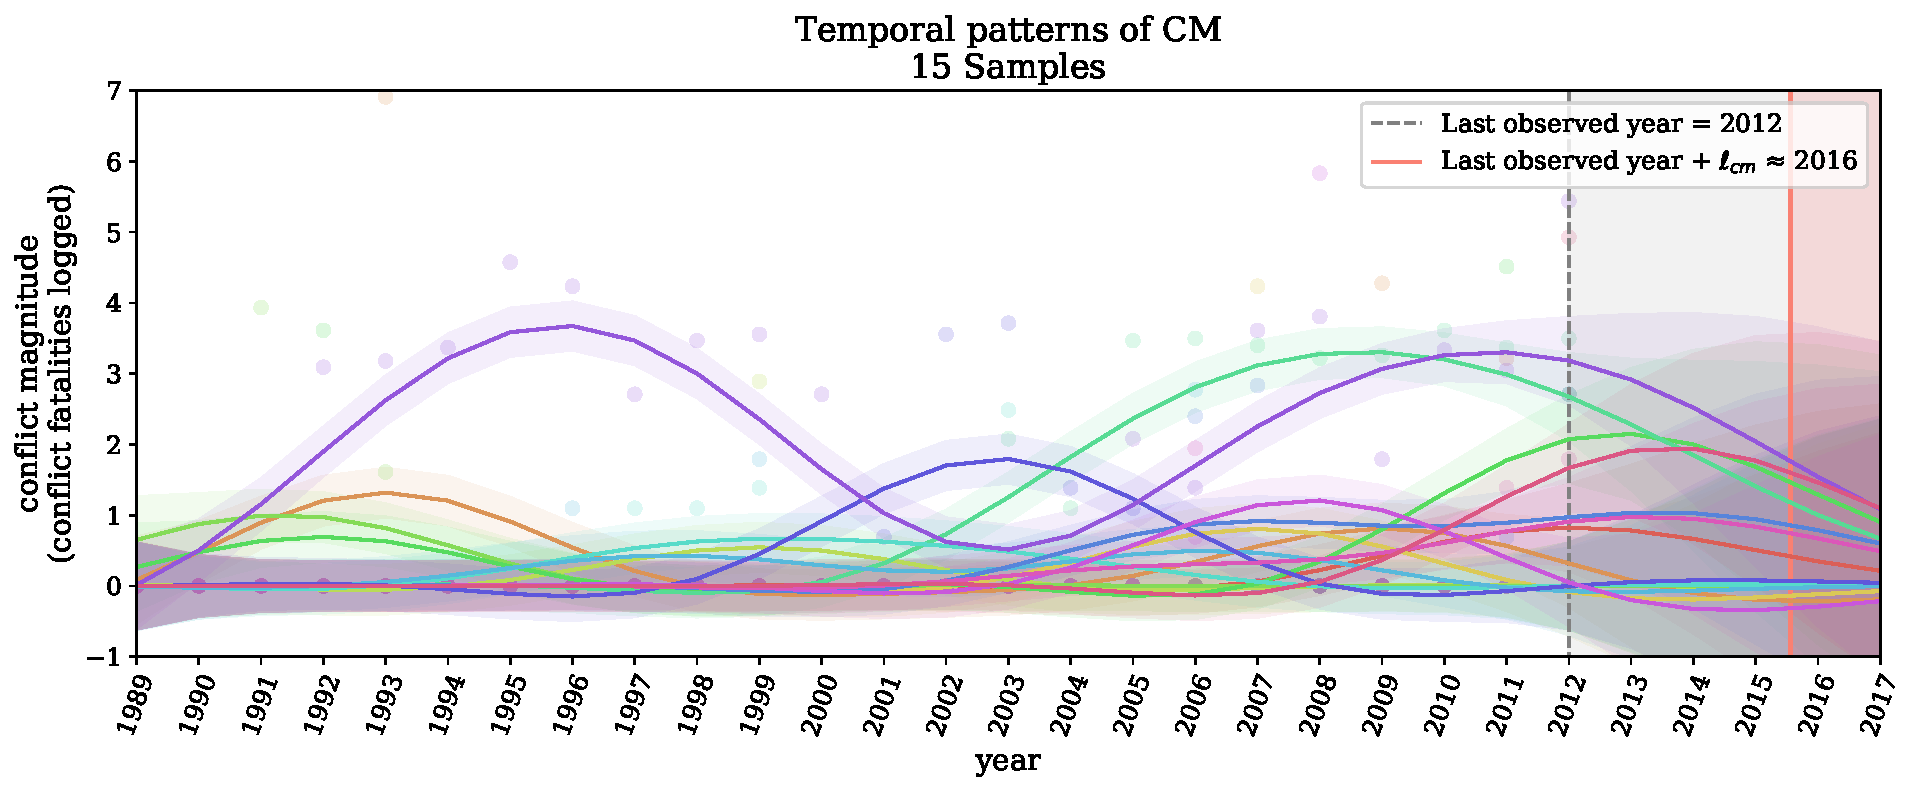
\includegraphics[scale=0.47]{cm_15_samples.pdf}
    \caption{\footnotesize{The estimated temporal patterns of conflict magnitude from fifteen randomly drawn time lines. For visualization purposes all fifteen samples has minimum one event over the course of the train years. The solid line is the maximum likelihood point estimate of $\mu_{cm}$ and the corrosponding shading denotes $2\times\sigma_{cm}$. At such, given them mocel there is a 95\% that $\mu_{cm}$ is within this zone. The scatter points are the actual observed values from the test set. $\ell_{cm}$ = 3.6, $\eta_{cm}$ = 1.1, $\epsilon_{cm}$ = 0.9}\label{cm_sampel_eks}}
\end{figure}

% Int. the samples
Turning to the estimated functions, I have extrapolated these beyond the train years into the test year simply by introduce $x_{yearNew}$. Using the estimated hyperparemeters and the data contained in the train set I now generate Gaussian processes for each time line across all years included in $x_{yearNew}$. This is what i illustrate in \autoref{cm_sampel_eks}. Here the estimated functions continues beyond the train years (1989-2012) into the test years (2013-2017) guided by past (training) data, the covariance ($k_{cm}$) function, the mean function ($m_{cm}$) together with the estimated error term and hyperparameters ($\epsilon_{cm}$, $\ell_{cm}$ and $\eta_{cm}$). As such, what I illustrate with the small sample in \autoref{cm_sampel_eks} is, that each of the functions estimated represents the temporal pattern of conflict magnitude pertaining to the time line of one specific grid cell. That is; how conflict have waxed and waned in each geographical cell over the course of the train years, and how this pattern can be expected to continue into the test years given data and model specification employed.\par

% What it does not capture: two steps ot ammend
What these functions does not capture however, is the spatial dimension of conflict. Just as conflict can move through time, it can also move through space. I need a measure capturing, not just the specific patterns pertaining to a specific cell, but also a measure capturing how exposed a said cell is to the conflict patterns of proximate cells. To create such measure I need to make two estimations. First I estimate a 2D Gaussian process for each year in the train set using longitude and latitude as features ($x_{lat}$, $x_{long}$: $X_{ll}$) and conflict magnitude  ($y_{cm}$) as target. This I call static conflict exposure ($sce$). This measure simply tells us how exposed a given cell is to conflict one given year without taking into account any temporal patterns. Secondly I also want this measure to capture the spatial patterns across time and to be able to extrapolate values into the furture. To achieve this I simply estimate a 1d Gaussian process as already done once. This time I again use year as the sole feature ($x_{year}$), but instead of conflict magnitude I use $sce$ as target. This give my a measure over all year for conflict exposure. This measure I call dynamic conflict exposure; $\tilde{y}_{dce}$. Instead of only taking into account the past pattern of the individual cell, this measure take into account the past patterns of all cells in the relevant vicinity.\par 

% SCE
As such, I first estimate the shared hyper-parameters and error term ($\ell_{sce}$, $\eta_{sce}$ and $\epsilon_{sce}$) for a 2d Gaussian processes pertaining to the spatial conflict patterns pertaining to each specific year in the train set. Conflict magnitude is my target $y_{cm}$ and I use longitude ($x_{long}$) and latitude ($x_{lat}$) as the features $X_{ll}$. This Gives me a measure of static conflict exposure $\emph{sce}$. It is "static" since I have yet to take time into account. The mathematical notation can be found in equations \ref{eq:form_sce}, \ref{eq:func_sce}, \ref{eq:m_sce} and \ref{eq:k_sce}.  The priors for $\epsilon_{sce}$, $\eta_{sce}$, $\ell_{sce}$ can all be found in the appendix [REF].\par

\[
\widetilde{log(CF)} = f_{sce}(X_{ll}) + \epsilon_{sce} \tag{23} \label{eq:form_sce}
\]

\[
f_{sce}(X) \sim \mathcal{GP}_{sce}(m_{sce}(X_{ll}),k_{sce}(X_{ll},X_{ll}')) \tag{24} \label{eq:func_sce}
\]

\[
m_{sce}(X_{ll}) = 0 \tag{25} \label{eq:m_sce}
\]

\[
k_{sce}(X_{ll},X_{ll}') = \eta_{sce}^2 exp\left(-\frac{|X_{ll}-X_{ll}'|^2}{2\ell_{sce}^2}\right) \tag{26} \label{eq:k_sce}
\]

% hyper parameters and sample
As before, I first estimate the hyper parameters and error term $\eta_{sce}$, $\ell_{sce}$, $\epsilon_{sce}$. I have no intention of extrapolating these patterns into unknown gepgrafical regions so I do not introduce any $X_llNew$.  The estimated hyper parameters and error term can be found in \autoref{sce_hp}. To visualize the output, the static conflcit patterns pertaining to 2012 are plotted in \autoref{sce_sampel_eks}.\par


% HP table
\begin{table}[!htb]
\begin{center}
\centering
% 	\begin{tabular}{l*{4}{c}}
	\begin{tabular}{m{3cm} m{3cm} m{3cm} m{3cm}}
	%\hline
	\textbf{Hyperparameters}\\
	\text{Static conflict exposure}\\
	\hline
                            &  \thead{Point estimate\\(mean)}   & \thead{Standard\\deviation}   & \thead{95\% Credibility\\interval} \\
	\hline
	$\ell_{sce}$             & \thead{x}        & \thead{x} 	& \thead{x - x}                             \\
    $\eta_{sce}$             & \thead{x}        & \thead{x} 	& \thead{x - x}                             \\
    $\epsilon_{sce}$         & \thead{x}        & \thead{x} 	& \thead{x - x}                             \\
  
    \hline
	\end{tabular}
\end{center}
\caption{\footnotesize{...}}\label{sce_hp}
\end{table}

\begin{figure}[!htb]
	\centering
	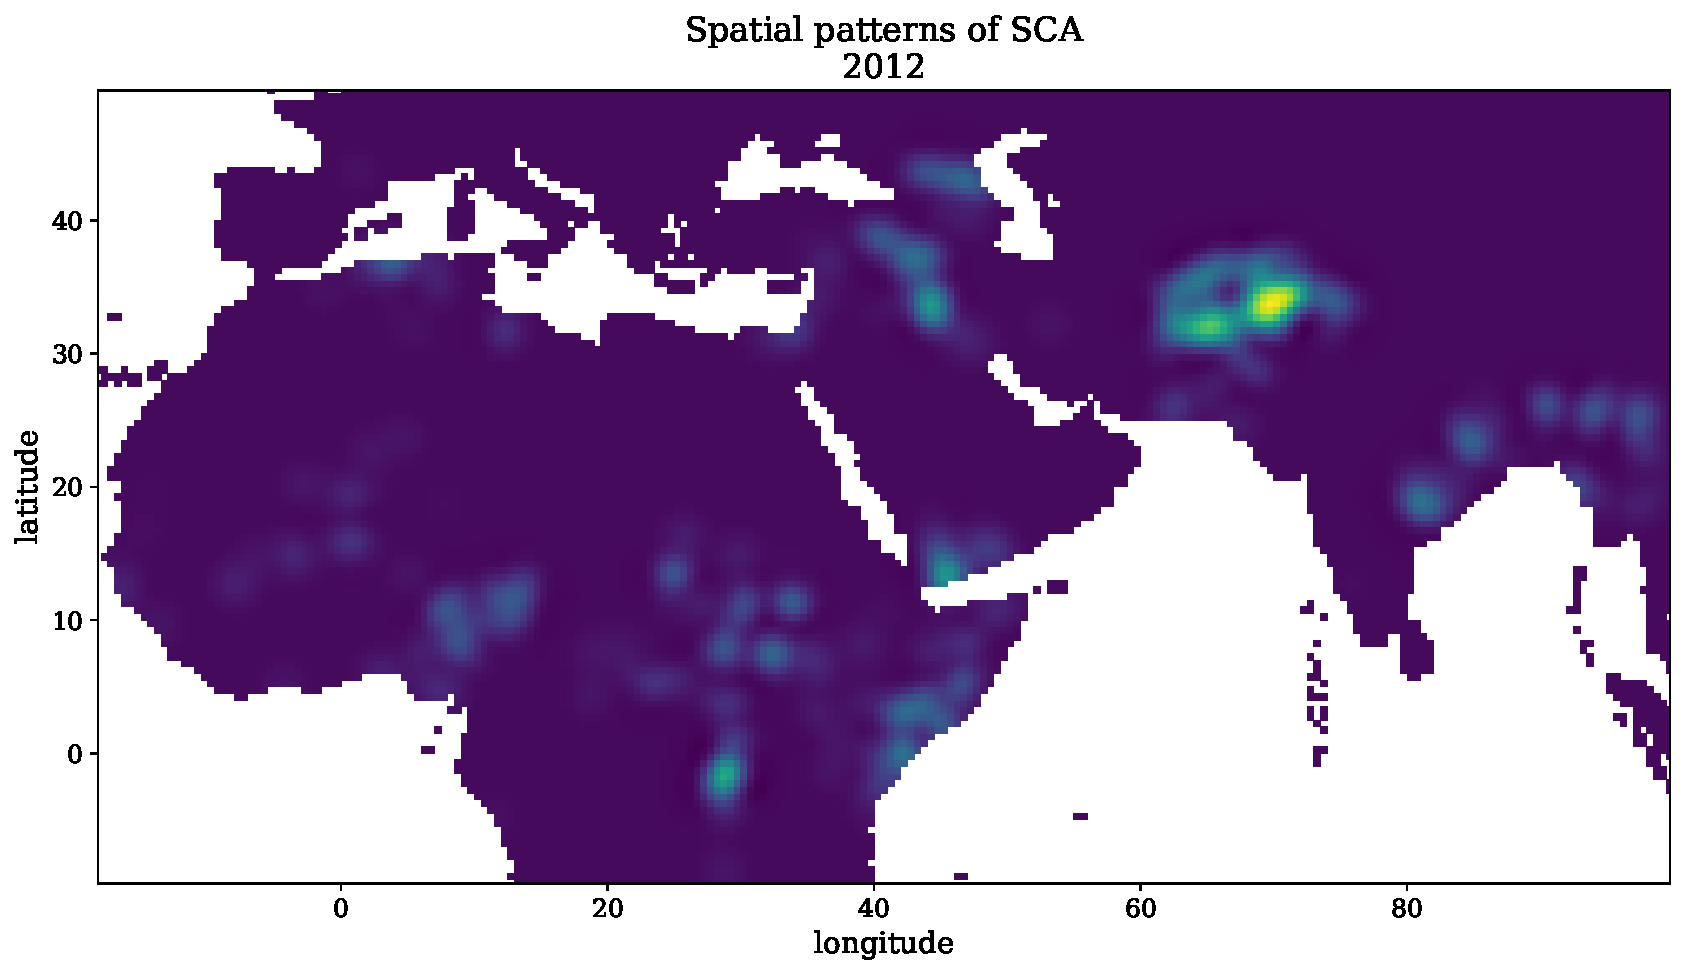
\includegraphics[scale=0.47]{sce_2012_samples.pdf}
    \caption{\footnotesize{}}
\end{figure}












% DCE
[OLD]
% int fig.



%These step will be implimentd below..













% OLD....
First, I estimate the shared hyper-parameters for a 2d Gaussian Processes pertaining to the individual spatial patterns for each year. I use logged conflict fatalities $CF$ as my target $y$. I use longitude and latitude as the features $X$ with the sub-indexing $ll$. This Gives me a measure of "static" conflict exposure $\emph{sce}$ - meaning I do not take time into account yet.\par

The priors for $\epsilon_{sce}$, $\eta_{sce}$, $\ell_{sce}$ are all weakly informative priors merely in place to encourage computational efficiency.\par

\[
\widetilde{log(CF)} = f_{sce}(X_{ll}) + \epsilon_{sce}
\]

\[
f_{sce}(X) \sim \mathcal{GP}_{sce}(m_{sce}(X_{ll}),k_{sce}(X_{ll},X_{ll}')) % \tag{5} \label{eq:f}
\]

\[
\epsilon_{sce} \sim \text{HalfCaushy}(3)
\]

With the mean function being the constant of zero and the covariance function being the squared exponential kernel function:

\[
m_{sce}(X_{ll}) = 0
\]

\[
k_{sce}(X_{ll},X_{ll}') = \eta_{sce}^2 exp\left(-\frac{|X_{ll}-X_{ll}'|^2}{2\ell_{sce}^2}\right) %\tag{7} \label{eq:k}
\]

\[
\eta_{sce} \sim \text{HalfCauchy}(1)
\]
\[
\ell_{sce} \sim \text{Gamma}(4,2)
\]


Note that I estimate and use shared hyper-parameters $\eta_{sce}$ and $\ell_{sce}$ for both longitude and latitude. This need not be the case, but since I have little theoretical reason to think that conflict spreads different across the two axis' this seems the prudent choice - which, incidental, is also more computational efficient.\par

On the the basis of the hyper-parameters and the data I can now draw samples from the posterior distribution pertaining to the static conflict exposure for each year. In this thesis I really only use the mean of these samples $\mu_{sce}$. This will be the target of the nest step.\par

%but it is informative to also extract the variance $$ for evaluation purposes.\par

Second, taking the value of $\mu_{sce}$ each cell across time effectively gives a time-line of static conflict exposure. To take time into account and to allow extrapolation into future years I now estimate a the hyper-parameters of a 1d Gaussian processes across each $\mu_{sce}$-time-line $dce$ in in trainset incorporating years from 1989 to 2014 [right?]\footnote{The reader might appropriately ask why I did not just estimate a 3d GP to begin with. Indeed, this would have been preferable, but the computational cost of adding more dimension raises exponential. Thus the computational resources at my disposal did not stand up to this challenge}. This gives allows my to estimate the \emph{dynamic conflict exposure}. As such, I use $\mu_{sce}$ as target $y$ and $years$ as feature $x$ with the sub-index $t$.\par

Again, the priors for $\epsilon_{dce}$, $\eta_{dce}$, $\ell_{dce}$ are all weakly informative priors in place to encourage computational efficiency.\par

\[
\widetilde{\mu_{sce}} = f_{dce}(x_t) + \epsilon_{dce}
\]

\[
f_{dce}(x_t) \sim \mathcal{GP}_{dce}(m_{dce}(x_t),k_{dce}(x_t,x_t')) % \tag{5} \label{eq:f}
\]

\[
\epsilon_{dce} \sim 
\]

And still the mean function is simply the constant of zero and the covariance function the squared exponential kernel function:

\[
m_{dce}(x_t) = 0
\]

\[
k_{dce}(x_t,x_t') = \eta_{dce}^2 exp\left(-\frac{|x_t-x_t'|^2}{2\ell_{dce}^2}\right) %\tag{7} \label{eq:k}
\]

\[
\eta_{dce} \sim
\]
\[
\ell_{dce} \sim
\]

Using the estimated hyper parameters and the data I draw samples from the posterior distribution. But instead of just drawing from the years used as features I extrapolated [X] years in the furture. Specifically the $x_new$ covers the the years from 1989 to 2017; that is both the years incorporated in the train and the testset.\par

Again here $\mu_{dce}$ is the estimate most interesting, but the estimate of the variance $var_{dce}$ also holds some nice information regarding how uncertain the estimates become when we extrapolate into furture years. To illustrate [figX] Shows the $\mu_{dce}$ of five different time-lines.\par

[figX]

As such $\mu_{dce}$ is one of the eight features to be used in the final prediction effort. 

% point elswhere: That fact that I have estimated values for the years in my testset, means that I don't need some rigid scheme involoving lagged features.\par

Moving on from dynamic conflict exposure to dynamic conflict magnitude $dcm$, the approach is very similar to when I estimated $\mu_{dce}$, but Instead of using $\mu_{sce}$ as target I use Logged(CF). Thus I do not here take any spatial dependency or diffusion into account. The Idea is that, while spatial diffusion is common, there might sometimes be a very good reason why a specific conflict does not spread from one cell to another.\par

These cell specific magnitude trends are more volatile than the dynamic exposure trend. To take this into account I tread the trend ad a product of two Gaussian processes instead of one: A long-term trend and a short term trend denoted respectively by the subscripts $lt$ and $st$. This is easily implemented as presented below.\par

\[
\widetilde{log(CF)} = f_{dcm\_lt}(x_t) + f_{dcm\_st}(x_t) + \epsilon_{dcm}
\]

\[
f_{dcm\_lt}(x_t) \sim \mathcal{GP}_{dcm\_lt}(m_{dcm\_lt}(x_t),k_{dcm\_lt}(x_t,x_t')) % \tag{5} \label{eq:f}
\]

\[
\epsilon_{dcm} \sim 
\]

The mean function for both the short term and the long term is the constant of zero and the covariance function for both short and long term is the squared exponential kernel function:

\[
m_{dcm\_lt}(x_t) = 0
\]

\[
m_{dcm\_st}(x_t) = 0
\]

\[
k_{dcm\_lt}(x_t,x_t') = \eta_{dcm\_lt}^2 exp\left(-\frac{|x_t-x_t'|^2}{2\ell_{dcm\_lt}^2}\right) %\tag{7} \label{eq:k}
\]

\[
k_{dcm\_st}(x_t,x_t') = \eta_{dcm\_st}^2 exp\left(-\frac{|x_t-x_t'|^2}{2\ell_{dcm\_st}^2}\right) %\tag{7} \label{eq:k}
\]

What is different here is natural that we get hyper-parameters pertaining to both a sort term trend and a long term trend. To achieve this I use some slightly more informative priors as presented below:

\[
\eta_{dce\_lt} \sim
\]

\[
\ell_{dce\_lt} \sim
\]

\[
\eta_{dce\_st} \sim
\]

\[
\ell_{dce\_st} \sim
\]

The priors are still not especially informative or coercive. Yet, I have defined the short term length scale $\ell_{dce\_lt}$ to be shorter than the long term length scale $\ell_{dce\_st}$. This is mostly for convenience, as it is my way of telling the framework with which of the two Gaussian processes I want to capture a potential long term and with which I want to capture a potential short term.\par

Regarding the amplitude $\eta$ [...]

% Importantly I am not forcing anything unnatural upon the framework; it will only find a discernible long - and short term trend if indeed the data support this proposition.\par

Figure [X] and [X] illustrates the division between the long- and the short term trend, while figure [X] illustrates the combined function.\par

[figX]
[figX]
[figX]

With $\ell_{dce\_st} = X$ the is not mush reason to extrapolated this trend into furture years. We can think of this as such: the short term trends are so unpredictable giving the data we use, that we can not foresee how they will behave in furture years. This dies not mean that we gain nothing from having estimated the two trends separately. Indeed we get a much larger $\ell_{dce\_lt}$ for the long term trend, then if we had only estimated one trend. And as we know a higher $\ell_{dce\_lt}$ allows us took look further into the future. 

Again I sample using $X_new$ from 1989 to 2017 As such what I use moving forward is $\mu_{dcm\_lt}$ as the feature capturing conflict exposure.\par




By now I


Since the short term trend only

From these trends I then derive the Slope, acceleration and mass through respectively differentiation and integration.\par

\subsection{Slope, accelaration and mass}



% Kommer direkte i forlængelse af Theory: Slutter af med fremgangmåde så læseren ved hvad der skal sker i analysen

% Below I briefly present the data and methodes utilized for the project at hand.

% HUSK: hvad er dine X (Z) i første omgang: year, lat long.
% Dine afledte X'er: Conflict Exposure and Conflict Proximity og F(X) (conflcit mass), f'(x) (conflcit slope) of f''(x) (conflcit accelaration/deccelaration) af begge disse alle forecasted in i fremtiden. I alt 8 features 


%\subsection{The Research Design and Methods}
% \todo[inline]{In the works}

% Her skal der også være om out of sample prediction (skal nævnes tidligere)
% Rare events. xgboost.  evaluerings matrix'er ect.


% Here I do not extrapolate into any unknown geography, but I could combine the two approach making a 3d Gaussian process the one pair of hyperparameters pertaining to the spatial dimension and an other to the temporal, ad then extrapolate the temporal pattern into the future. One challenges I encounter here is unfortunately computational limitations. Again, i shall not get to technical, but the computation needed grows exponential with the number of dimensions \citep[503]{Gelman_2013}. I this endeavour I bypass this problem by simply taking one step at a time. First estimating the temporal pattern in 2d for each year then, estimation the temporal dimension of the spatial patterns using this data in 1d. This is not true 3d, but it comes rather close, not least since I do not expect observations removed far from each other in both time and space to be correlated anyway.\par



% en fordel ved at de er smooth er at de kan differentieres

\subsection{Second layer: Predicting conflicts}
\todo[inline]{todo}

\section{The Results}
% [Analysis]
% I virkeligheden mest bare resultaterne; start bare hård med et resultat.


\section{The Conclusion}

\section{Futher Perspectives}

% if you want arguement regarding baseline model look at \cite{schutte2011diffusion}.



% +++++++++++++++++++++++++++++++++++++++++++++++++++++++++++
% OLD +++++++++++++++++++++++++++++++++++++++++++++++++++++++
% +++++++++++++++++++++++++++++++++++++++++++++++++++++++++++


%\section{The Challenge}

%The goal of this master thesis is to add knowledge to the growing field on computational conflict prediction\footnote{Aka. the creations of reliable early-warning-systems}. By conflict I here refer to the following definition from the Uppsala Conflcit Data Program (UCDP):

%\begin{displayquote}

%\emph{"An incident where armed force was used by an organized actor against another organized actor, or against civilians, resulting in at least 1 direct death at a specific location and a specific date."} \citep{Croicu_Sundberg_2017}

%\end{displayquote}

%More specifically the focus of my project in intrastate conflicts. Thus I limit my self to cases where only one of the included "organized actors" is a country. Appropriately I therefore also takes as the unit of analysis sub-national unites; specifically geographical cells of $0.5 \times 0.5$ decimal degrees derived from the PRIO grid database \citep{Tollefsen_2012}, which I shall return to in \autoref{data}.\par 

%As rather novel field, conflict prediction is faced with a plethora of challenges to be tackled before a appropriately reliable early-warning-system can be constructed\footnote{Unless, of course, conflict is inherently shrouded in ontological uncertainty rather than epistemology uncertainty as implied by \cite{Gartzke_1999} in which case the field should be abandoned - luckily results from the last ten years inspire optimism.}. One of these challenges is creating a coherent framework for modeling the temporal/spatial diffusion-pattern of conflict. To clarify, most efforts of conflict predictions are constructed as a econometric or machine-learning problem and include as predictors various features pertaining to all sorts of phenomena. All with various proposed theoretical links to the process of conflict. These phenomena stems from the litterateur on greed, grievances, resource courses and so on. Two closely related dimensions which often also finds themselves included in prediction efforts are the fundamental dimensions of time and space. These dimension have been included both to combat temporal and spatial auto-correlation\footnote{ often using some fixed, random or conditional effects}, but also to capture more complicated phenomena such as \emph{conflict traps} and \emph{conflict diffusion}. Specifically regrading conflict traps and inertia \cite{Collier_Hoeffler_2004} uses a linear decay function counting years since last conflict; \cite{Hegre_Sambanis_2006} uses a linear decay function counting years since last peace; \cite{Cederman_Gleditsch_Buhaug_2013} count the number of previous conflicts; and \cite{perry_2013} propose a "deterioration index" counting the number of fatalities in a given year and diving with the number of years since said given year. Meanwhile, cross-country dispersion has been modeled by \cite{Goldstone_2010}.\par% mere med diffusion!

%These efforts have contributed with important insight, but while they have included features aimed to capture the temporal/spatial pattern of conflict this have not been their prime focus. The consequence is that the features meant to capture these dimensions often appears ad hoc and both methodologically and theoretically underdeveloped. This is further exemplified by the fact no consensus regarding how these dimensions should be modeled have emerged. This is where the present thesis aims to contribute.\par

%This thesis concerns itself only with modeling conflict as a function of conflict in it self. Where conflict have been before and where conflict is now. Crucially the goal is to create a unified methodologically and theoretical coherent framework for the creation of features pertaining to the diffusion of conflicts in time and space based on modern computational methods. To add some much needed context to this rather lofty goal, let my exemplify the challenge at hand by referencing the deterioration index proposed by \cite{perry_2013}. Perry's idea is somewhat connected to the phenomenon of a conflict trap and the notion of some inertia in conflict induced grievances: people want revenge, but the lust for revenge might deteriorate over time. The time deteriorating index would be created by including the number of fatalities in some geographic unit for each of the last ten years as features. The idea is then to down-weigh these fatalities by dividing with the number of years past since the corresponding events. Thus, a feature pertaining to fatalities two years ago will have, as its values, half of the fatalities observed that year \cite[14]{perry_2013}. While the heart is at the right place, it is an ad hoc and underdeveloped solution. There is no reason to cap the effort at ten years and there is no theoretical or practical reason to choose the suggested deterioration rate. Instead of dividing with years past it might be more appropriate to multiply by 0.8 or 0.2; or the deterioration rate might have an altogether different functional form, like an exponential or linear decay function as proposed by \cite{Collier_Hoeffler_2004} or \cite{Hegre_Sambanis_2006} - in which case we still need to decide (read guess) some appropriate deterioration rate. And how are we to translate this index if we change time unite to months or weeks? The crucial point is that we do not know the function(s) and therefore we should estimate the function(s). Also, estimation at least gives us some indication of how bad our "guess" is.\par 

%The exact same problem is present in the context of spatial diffusion. \cite{Goldstone_2010} finds that sharing border with four or more conflict ridden countries increases a given countries risk of civil war and democratic breakdown significantly \cite[195]{Goldstone_2010}. Surely there must be differences in regards to the size of the bordering countries, the severity of the conflict and where in the neighbouring countries the conflicts occur. Further more time and space most interact in some way or another. Meaning that persisting conflict could be more likely to spread or, as argued by \cite{bara_2017}, the termination of conflict in one place might to push weapons and combatants to a neighbouring regions \cite[2003-2006]{bara_2017}. Again the point i clear: modeling features to capture these phenomena is an should be an estimation effort in it self.\par 

%The tools I propose to use for this estimation effort are presented in the next section, while the corresponding data is presented in \autoref{data}.\par

%\section{The Methods}

%There are a number of steps involved in this project, but the two most crucial are feature engineering and evaluation through out-of-sample prediction. Importantly the feature engineering part is here also a estimation effort and will be the prime focus of the project. The preceding prediction effort will serve simply to evaluate the potential of the feature space created; a feature space only pertaining to the temporal/spatial dimension of conflict. I will present each in their own subsection below.\par

%\subsection{Creating the Temporal/Spatial Feature Space}

%The machine learning technique of \emph{Gaussian processes regression} have been used to model both temporal and spatial dependency in Bayesian multilevel models with good results before \citep[411-419]{Mcelreath_2018}. To illustrate via a very simplified and non-technical example: most political scientist are familiar with fixed, random or varying effects models which can facilitate more or less individual intercepts and slopes for each observation according to a categorical scheme such as \emph{country}, \emph{decade}. Including Gaussian processes allows intercepts and slopes for each observation according to a continuous scheme, such as distances like \emph{miles} or \emph{years}. Intriguingly combining these approaches allow the rate of conflict diffusion to differ across countries and regions\footnote{Or indeed any other geographical unit} \citep{gelfand2003spatial, gelfand2012hierarchical, gelfand2016spatial}. The visual toy-example in \autoref{gp_eks} will serve to illustrate the approach further.

%\begin{figure}[!htb]
%	\centering
%	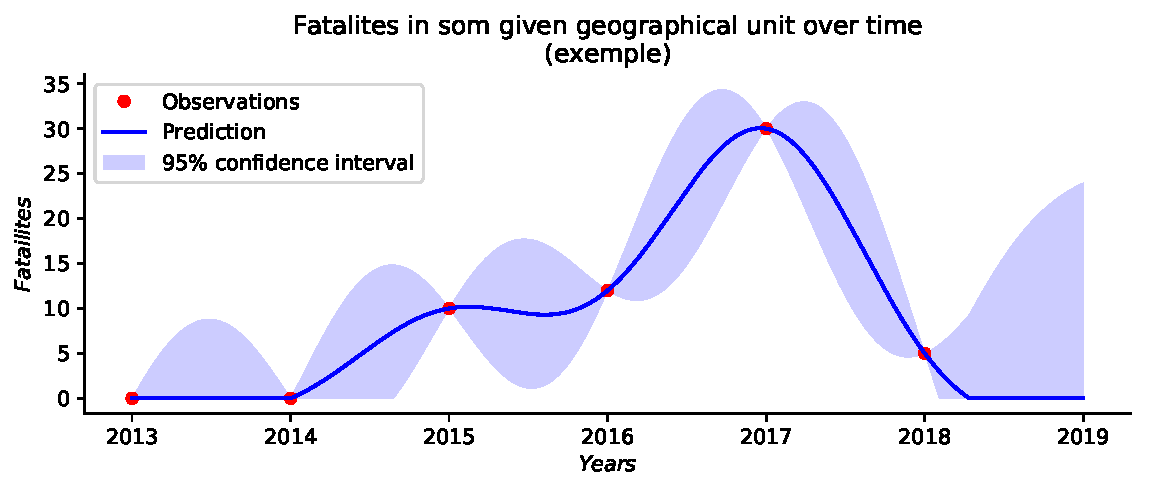
\includegraphics[scale=0.7]{GP_eks.pdf}
%    \caption{\footnotesize{Gaussian process regression regarding the development in conflict fatalities over time in some given geographical unit.}}\label{gp_eks}
%\end{figure}

%\autoref{gp_eks} illustrates a simple example. Imagine some some given geographical unit - like a PRIO gird cell. We are give yearly fatalities corresponding to the years from 2013 to 2018. You are tasked with estimating the number of fatalities in 2019. This is exactly what the Gaussian process regression above does. Its best estimate is 0 fatalities as it recognized the negative trend. However it "remembers" from past experience that the cell do have conflict potential; this is seen in high uncertainty reflected through the confidence interval pertaining to 2019. As such \autoref{gp_eks} illustrates not just the approaches capabilities in regards to modeling patterns of diffusion, but also it ability to estimate uncertainty and the fact that it is geared towards forecasting challenges. That is, we could just as well have asked for the estimated fatalities count in 2020 or 2021. These estimates will no doubt be clouded in uncertainty, but it is an estimated uncertainty representing our current knowledge of the cell.\par

%Naturally the x-axis could readily be replaced the coordinates for longitude or latitude\footnote{Or other appropriate spatial unites} and temporal dispersion would be neatly modelled. Creating a 3 dimensional space of years, latitude and longitude would yield a geographical map for each included year where information regarding the pattern of conflict would be shared between all three dimensions. Whether the final feature space should be represented as one, three or more features is an empirical question I have yet to answer. Never-the-less, the fact that both the temporal and spatial patterns have potential of being modelled according to a unified approach is both practical and encouraging.\par\par

%As mentioned, however, these predictions are to be features not final predictions. A smaller doll in a babushka doll of predictions if you will. The actual prediction framework in which the features will be tested is briefly present in the next section.\par

%\subsection{Evaluating the Feature Space Through Prediction}

%One of the greater challenges pertaining to conflict prediction is the imbalance of the data; most of the time, most grid cells do not experience any conflict fatalities. The data as such is greatly imbalanced. To handle this challenge I use a suitable estimation procedure, I under-sample the non-events and I utilize the appropriate evaluation metrics. These framework is a bit comprehensive, so I will only be presenting the bare bone intuition below.\par

%\subsubsection{Extreme Gradient Boosting}

%I utilize the Extreme Gradient Boosting (xgboost) algorithm as the basis of my predictions \citep{Chen_2016}\footnote{Implemented through python}. This method is a bit advanced and I shall refrain from digging into the technicalities of the algorithm. However, some fundamentals serve to explain why this framework is especially well suited for the problem at hand. Three characteristics needs presenting; it is a boosting algorithm, it is consisting of regression trees and it is self-regularizing (or self-pruning).

%Boosting involves using a lot of weak classifiers to create a strong classifier. Imagine that we begin with one classifier with which we try to classify geographic locations which will experience conflict fatalities next year. The classifier does rather poorly, not least due to the fact that the events are few and and hard to classify. Thus, we decide to run a new classifier, but now we give less weight to the observations which was correctly predicted and more weight to the observations which was incorrectly predicted. We reiterate this procedure until some measurement criteria is met. Then, all our classifiers are weighted according to their performance and used as a weighted ensemble to predict which geographic locations will experience conflict fatalities of the following year \citep[338-339]{Friedman_2001}. Since the procedure ensures continuing focus on "hard to classify" observations, it is a particularly fruitfully approach when dealing with imbalanced data.\par

%The Next question is naturally which classifiers to build our boosting framework on. Xgboost utilizes regression tree. These closely resembles decision tress where the features are used to split the observations into categories according to which splits yields the most information according to some predefined criteria. Thus, the first split would here be the split which best sorted conflict events from non-events and so on. But unlike decision trees, each regression tree holds a continuous score on each of the leafs, which can be converted into probabilities rather then binary classifications \citep[2]{Chen_2016}. To put it simply, xgboost utilizes N number of regression tress and iteratively uses the predictions of one tree to update the weights of the next tree, such that 'harder to classify' observations are given continuously more and more attention.\par

%The last question here is then how to decide to number of times we shall allow a given tree to split. Too few times and the tree fails to learn any pattern of the data and we underfit. To many splits and the tree starts to learn idiosyncratic artifacts of the training data and we overfit. The xgboost algorithm handles this by penalizing complicated tress. Thus, when the algorithm evaluates whether or not to make a split, the information gain obtained by the potential split is down-weighted according to the increased complexity induced by new splits \cite[4-7]{Chen_2016}. Thus, the algorithm searches for any patterns which might help the prediction effort, but stops before such pattern becomes overly complicated.\par 

%Naturally there is more to the xgboost algorithm than presented here, not least the fact that it has been optimized for sparse data in a number of more technical ways making it even more suited for large and imbalanced data-set then other boosting algorithms \cite[5]{Chen_2016}. Furthermore, the algorithm has a plethora of hyper parameters which will be tuned and optimized to further enhance performance and reduce overfitting\footnote{Usually optimized using k-fold cross validation \citep[241-249]{Friedman_2001}}.\par 

%\subsubsection{Undersampling}

%While the boosting approach presented above is able to handle imbalanced problems, we can help it along by re-sampling our training data to create a more balanced ratio between events and non-events. This is called undersampling \citep[1266-1267]{He_2008}. The specific procedure employed here is called \emph{case-cohort sampling}. I utilizes all available events from the trainingset along a random subset of no-events from the trainingset in order to construct the classifiers used \citep[142]{King_Zeng_2001}. The actual probabilities estimates are, however, inflated since the model thinks that conflicts are less rare than is the actually the case; this is corrected using Bayesian prior correction closely related to what is presented in \cite{King_Zeng_2001}, \cite{king_zeng_2001b} and \cite{Goldstone_2010}.\par

%While most of the information in the data is stored in the events and not the non-events \cite[139]{King_Zeng_2001}, some information is still lost by not using all non-events. The chosen solution is a variant of \emph{informed undersampling}. To counter the inefficient use of information, one can use an ensemble of classifiers all utilizing a new independent subset of non-events to combine with the subset of all available events \cite[1267]{He_2008}. This approach not only utilizes all information available, but also facilities the estimation of the uncertainty inherent in the prediction effort.\par

%Some initials have shown that such a framework do even better if the incoming test data is balanced in accordance with the training data used to create to models. Naturally, such a test is only possible because I do a test-set for evaluation purposes; which of course does not match any practical real world forecasting scenario. However, one could take some precautions. We could weed out all countries or cells which have never experienced any conflicts in our data sample and which are also relatively far from any ongoing conflicts. This would reduce the number of non-events substantially, thus making the incoming data less imbalanced.\par

%An other similar solution would be a "zero-inflated" framework with two or more rounds of estimations. The first round would correspond with the present endeavour. The second round would only include cells with a predicted probability over some appropriately low minimum threshold of conflict risk e.g. 1\%. This is more computational burdensome than simply sorting by country, but it is also more systematical and potential more powerful.\par 

%\subsubsection{Evaluation}

%I will again refrain from digging into this matter in full. The small snippet below will sufice for now.\par 

%Many metrics are available, but the most commonly known are probably "Accuracy", "Receiver Operating Characteristic" curve and the related measure "Area Under the Curve" (AUC) scores. While accuracy is intuitively meaningful and the ROC/AUC score has been coined as a "gold-standard" \citep[366]{perry_2013}, these measures also have some inherent limitations in regards to the specific problem at hand. Accuracy is not very suited for imbalanced data \citep[1264]{He_2008}. The ROC/AUC score tend to judge performance on highly imbalanced data too favorable \citep[1278]{He_2008}. I instead utilizes the metrics "Recall" and "Precision" along two closely related ratio metrics; the "Precision-Recall Curve" and the "Average Precision Rate". These measures are suitable for imbalanced data; have a substantial and conveyable interpretation; judges the present framework appropriately honest and harshly; and with the ratio metrics we circumvent the problem of a hard threshold \cite[1278]{He_2008}.  \par


%\section{The Data}\label{data}

%Below I briefly present the data utilized for the project at hand.


%\subsection{UCDP}

%Most central to the endeavour at hand is the data regarding intra-state conflict itself. This data is obtained through the Uppsala Conflict Data Program (UCDP) \citep{Sundberg_2013, Croicu_Sundberg_2017}. Specifically I utilize the UCDP Georeferenced Event Dataset (GED) Global version 18.1 \citep{UCDP_2017}. The dataset contains records of conflict fatalities and the corresponding coordinates and dates. I utilized data from 1989 through 2017 or 2018 if it becomes available doing the spring\footnote{For a smaller less detailed feature space data is available going back through 1975}. 

%as mentioned the project at hand limits itself to intra-state conflict, thus I only included incidents which do \emph{not} include two different nations as the organized actors. This data source provides both the prediction target and all information most information for feature engineering. I plan to estimate both probability of conflict and fatalities count on yearly basis.

%\subsection{PRIO}

%The PRIO grid is a global grid divided the world - excluding Greenland and Antarctica - into grid cells of $0.5 \times 0.5$ decimal degrees. It is constructed as geo-spatial (vector) data and primed for collaboration with the UCDP data. As such merging and handling these two data source is a trivial task. Again, to foster an intuitive understanding of the matter at hand is illustrated in \autoref{log_conflicts_2007}.

%\begin{figure}[!htb]
%	\centering
%	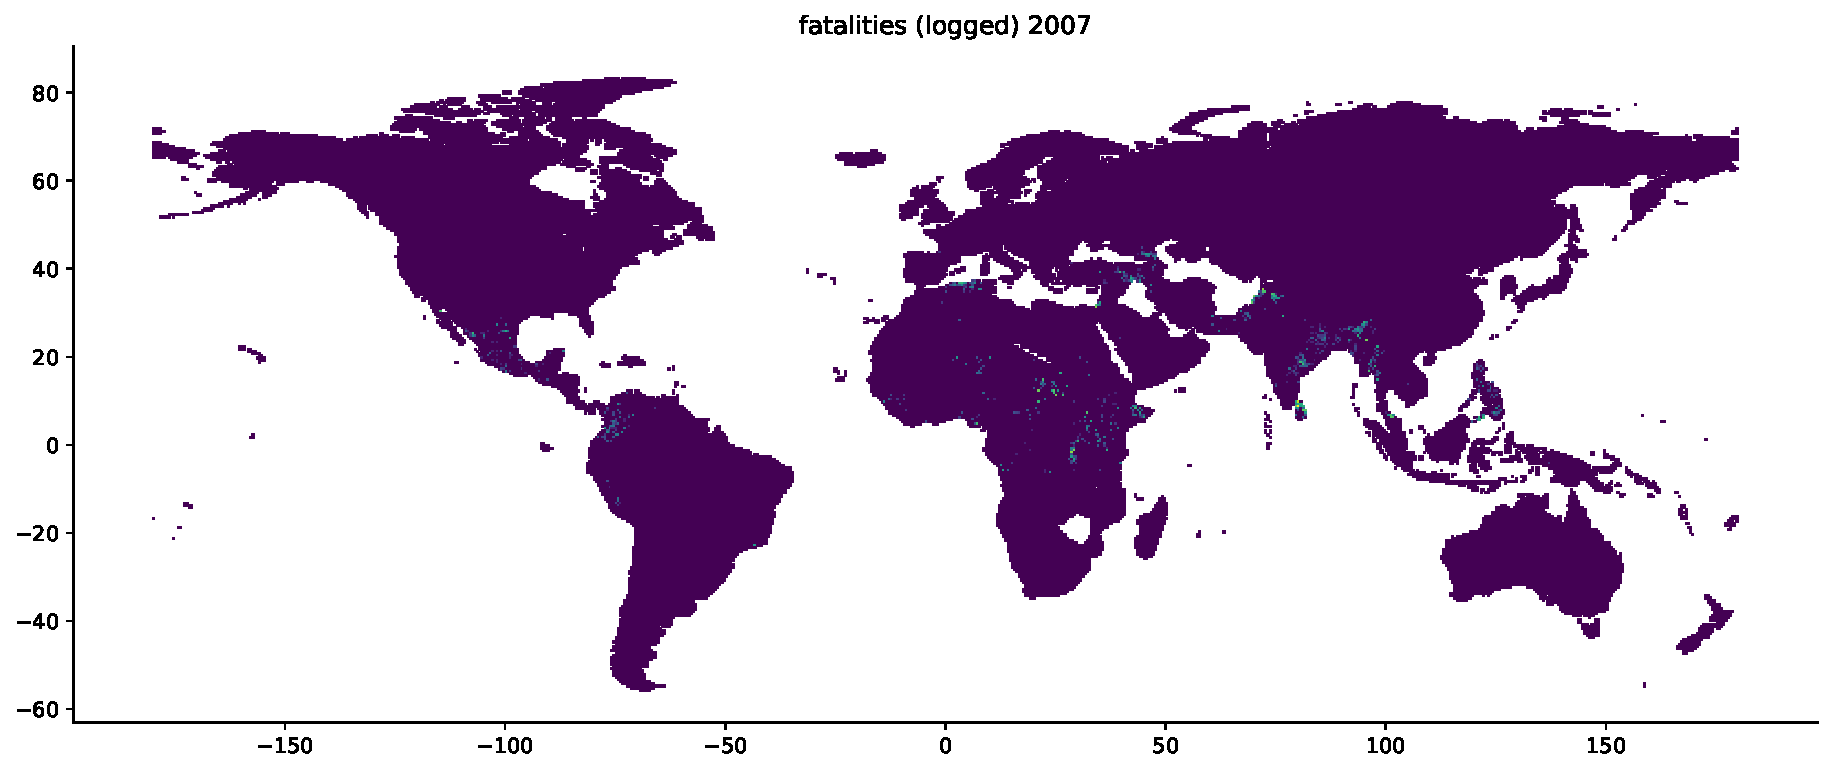
\includegraphics[scale=0.5]{log_conflicts_2007.pdf}
 %   \caption{\footnotesize{Conflict fatalities (logged) from 2007 according to UCDP %aggregated at the level of PRIO grid cells. Afghanistan, Iraq, Turkmenistan, Georgia and %Zimbabwe are missing this year due to the coding rules of UCDP.}}\label{log_conflicts_2007}
%\end{figure}

%Here we see the conflict all conflict fatalities classified by UCDP in 2007 aggregated from coordinates to PRIO grid cell level. Notably, while it may appear to be raster data each squared cell is indeed a vector with all what that entails regarding geospatial operations.

%\section{Last Remark}

%Thanks for reading. While it is a bit hastily compiled I do hope the above makse some sense and I look forward to your feedback.\\
%Best regards\\
%Simon


\pagebreak

\section{Bibliography}
\bibliographystyle{apalike} 
\bibliography{conflict.bib}

\section{Appendix}

[...]

%\subsection{Visual illustration of Gaussian distribution and Gaussian process}\label{GDGP}

[...]

\end{document}
